%ANDY Just a comment on this paper. The updated background on PIRGS can be further integrated and substitute the one now in other papers to be submitted as well as in the introduction of the thesis. I did not go through this chapter which seems the paper that we still have to fix.

\chapter{Using social interaction analysis and deception for entertainment support in a physically interactive robogame}\label{ch:deception}

A game is an activity that one engages in for amusement. In the quest for new playing experiences, robots are being developed to take part in interactive games with humans. Making believable, playing robots able to keep human players engaged and satisfied with the playing experience is the main challenge for this kind of applications. 
With this research aim, this paper investigates the quality of interaction between a human player and a mobile robot in a physical, interactive robogame. We apply previous development in social interaction analysis and, in particular, we focus on the applicability of deception theory as a mean to support engagement. By analyzing the social situation between two players (human and robot), identifying the need for deception, and acting upon it, we aim at decreasing predictability while increasing engagement and amusement, which are related to the perception of an opponent smart enough to compete at the right level. Experiments have been conducted on a population of 93 people which have been asked to play the game and answer a questionnaire. The majority of the participants enjoyed the game and perceived the robot as a rational agent that aims to win the game. Deception was also perceived by most of the players.

\section{Introduction}

As technology grows, the amount of devices that are part of our daily life rises as well. Since childhood, the new generations are learning to interact with technology while playing with new games implemented in embedded systems. This phenomenon can be seen on a large scale with robot games. New researches are made on robots developed to interact with human players in a game environment. Games not only make people have fun, but they are one of the most powerful tools for socialization, and cognitive development~\cite{vygotsky_play_1967, bruner_play:_1976, piaget_play_2013}.  While playing competitive games, a person is encouraged to learn the opponent's behavior for various reasons; for example, having a good knowledge of the opponent's behavior is essential for building a winning strategy, and this plays an important role in creating amusement.

%\begin{figure}[htbp]
%\centerline{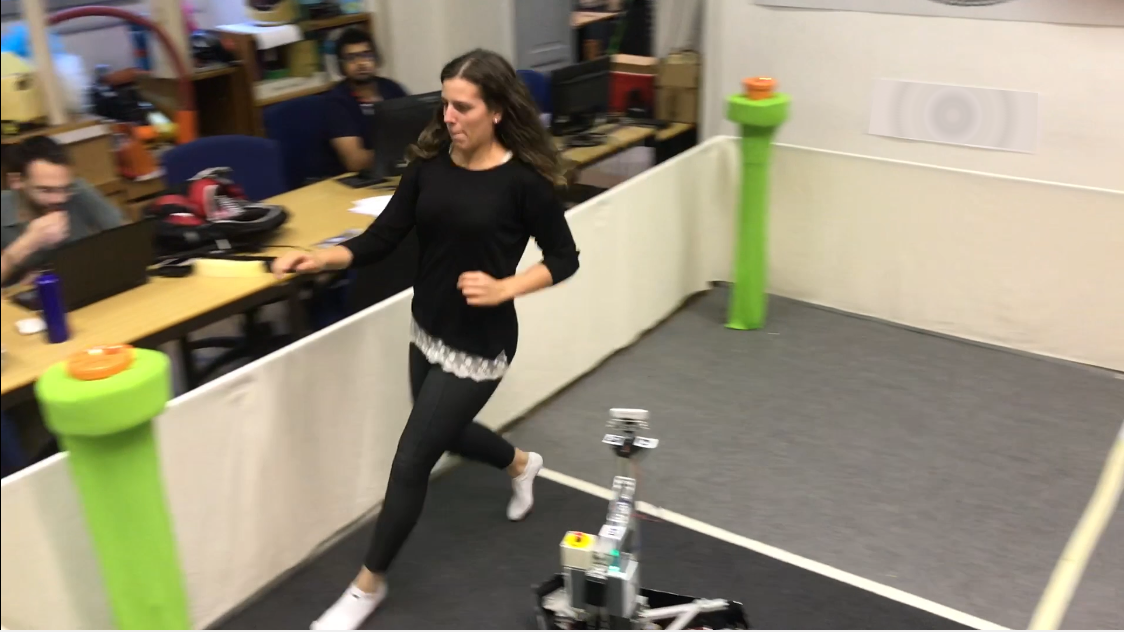
\includegraphics[width=0.5\columnwidth]{images/06-deception/frontPaper23}}
%\caption{Human-Robot interaction scene from our experiments.}
%\label{fig::front}
%\end{figure}

The main issues that should be faced in this field concern the robot's intelligence as perceived by the human player: low or too high levels may induce the player to leave because the robot is not considered as a valid competitor, and this lowers the entertainment level of the game. 

We are focusing on a challenging type of games, where the players are involved in a physical, quite demanding activity. This type of games has been introduced as~\gls{pirg}~\cite{martinoia_physically_2013}). In~\gls{pirg}s, it is important to model the player, by using the only available data that could describe well enough the movements of the player.

In different and not physical games, deception has been recognized as a way to increase attributions of mental states to the robot\cite{shim_taxonomy_2013}.

Our research aims at analyzing human-robot interaction in games. More  precisely, we try to improve the study on conflicting games, where the use of intelligent strategies by the players is the main path for winning the game. Deception is one of these strategies and it is not trivial communicating it to a human being using a robot. Our work gives a baseline for detecting and communicating deception in PIRG applications.

To the best of our knowledge, this is the first research work that applies deception theory to support engagement in a PIRG with mobile robotic platforms. 
The paper is organized as follows. Section~\ref{S:RelatedWorks} introduces related works, section~\ref{S:Thegameenvironment} explains in details the game, in section~\ref{S:Method} the method for detecting the need of deception and how to translate it into motion activity are described, experiments and validation of the proposed method are presented in section~\ref{S:Validation}, finally, discussions and conclusions are discussed in sections~\ref{S:Discussion} and~\ref{S:Conclusion}.

\section{Related Works}
\label{S:RelatedWorks}

\subsection{Deception and robots}
Interpersonal situations and interaction between individuals have been studied in sociology. Interdependence theory has been introduced in~\cite{kelley_interpersonal_1978}, where the authors studied the fact that people adjust their interactive behavior as consequence of their perception of a social situation. The adjustment is dictated by rewards and costs that every choice in a determinate moment in time can lead to. Every situation, then, can be expressed as a multiple choice of rewards in a matrix form, called outcome matrix. This concept can be seen as an equivalent game theory's normal form game. Furthermore, the authors introduced a four dimensional space where mapping of social situation occur using the constructed outcome matrices. Interdependence, correspondence, control and symmetry are the four dimensions that define that space. The first two respectively represent how much individuals influence each other reward and if outcomes of the individuals are consistent. 
An algorithm for analyzing social situations for robot's interactive behavior that uses the interdependency theory proposed in~\cite{kelley_interpersonal_1978}, is described in~\cite{wagner_analyzing_2008}. Our proposed method takes inspiration as well from~\cite{kelley_interpersonal_1978}, but in opposition to~\cite{wagner_analyzing_2008}, revisits the interdependence space (only 2D space interdependence-correspondence) and the way of mapping the outcome matrices as it will be discussed in Section~\ref{S:Method}.
In~\cite{wagner_robot_2009} an algorithm for detecting when and whether a robot should deceive has been proposed; the decision is based on the mapping of the outcome matrix to the interdependence-correspondence space. This algorithm has been used in~\cite{wagner_acting_2011}, where the analysis of the social situation is performed to provide robots with the capacity of determining if deception is needed. 

%MORE INFO: Experiments with the robot that has to choose between 3 paths and it has to deceive in a sense of leaving a false hint of where it passed by; the experiments confirm that outcome matrices can be used for detecting if deception may be needed, but it is focused on other individual's model.
The works of~\cite{kelley_interpersonal_1978, wagner_analyzing_2008, wagner_acting_2011, wagner_robot_2009} have laid the foundation for many research activities in social aspects involving humans and robots, in particular on the aspect of \textit{deception}. From the taxonomy in~\cite{shim_taxonomy_2013}, it is possible to classify deception according to the interaction object. Objectively, there are two types of deception, human-robot and nonhuman-robot.
An example of nonhuman-robot deception is~\cite{shim_biologically-inspired_2012}, where a squirrel-robot was capable of deceiving another one for gaining more food.
On the other hand, deceiving a human is not trivial. Studies about a robot able to deceive a human have been reported in~\cite{terada_can_2010}, where the authors discuss whether the feeling of being deceived by a robot would be an indicator that the human treats the robot as an intentional entity. 
%MORE INFO: The experiments have been conducted by producing a behavior against the human being's prediction. The robot is only able to rotate on its position for playing 'UN DUE TRE STELLA'. [Andrea] Either we will describe the experiment or I would not mention this.These experiments are not in a playing context.
Further experiments about the engagement increasing in a game due to a robot able to deceive, have been conducted in~\cite{short_no_2010}. This cheating 'rock-paper-scissors' interactive robot takes advantage of the deception for its own benefit.
%MORE INFO: the robot cheats in the 'rock-paper-scissors' game changing its choice after seeing the opponent's one and changing in its own favor the final result of the game. The authors find that it is noticeable the increased level of engagement by the participants when the robot cheats.
Differently from that robot, the robot presented in~\cite{vazquez_deceptive_2011} has been programmed for following a multi-player, reaction-time and conflict game, where its main role is to establish who is winning. The robot does not play, but it sometimes changes the wons in order to make the game more social engaging when the players discovered the cheating behavior of the robot. %TODO I can hardly see how the game might become more interesting when cheating of the robot is discovered.
%[EWERTON], this is really strange.

The most important part in a deceiving algorithm is to properly transmit to the deceived the false communication. This is a delicate part because the deceived should not understand it is under deception. 
In~\cite{dragan_analysis_2014} the authors propose a way to study the communication of false information (deception) using a robotic arm. On the work, the author reinforce the applicability of robot deception in making games against robot more engaging. All the paper is concentrated on robot deception in goal-directed motion, by learning deceptive trajectories in which the robot is concealing its actual goal. The present work is similar to ~\cite{dragan_analysis_2014} in the sense that it also explores goal-directed motion by following trajectories, but differ from that work on using a full mobile robot in a real game scenario. 

%TODO Actually, this method has not been presented and it seems a completely different context. Let's write what are the similarities.

%[EWERTON] -> improved the description without digging in on the description of the method.

\subsection{Physically Interactive Robogames}

Robot toys are presently the largest amount of robots delivered in our homes, at a rate of millions every year. In almost all the cases, the interaction is limited to stimulus-response reactions, but the introduction of low-cost sensors and computer power are making it possible to introduce a richer interaction and games specifically designed for mobile robots. In a PIRG, physical autonomous (often mobile) agents are actively engaged in a game that creates some sort of interaction, either competitive or cooperative, between humans and robots, moving in the physical world. Robogames will be one of the next robotic products for the mass technological market, thus demanding a large exploration of new methodologies and applications, especially for what concerns methods for enabling high autonomy, intelligence, and adaptive behavior, in order to respond to demands in engagement support like the ones expressed in~\cite{yannakakis_entertainment_2008,yannakakis_how_2008,yannakakis_real-time_2009}. 
Being able to evaluate how people play is crucial for an adaptive game. In the virtual game industry, several studies have been published, most of them using artificial intelligence and machine learning algorithms. For instance,~\cite{drachen_player_2009} reports about emergent self-organizing maps for grouping types of players. 

There have been attempts for presenting robots as toys over the years, where, in most cases, the robot acts more or less like a mobile pet (e.g.,~\cite{fujita_open_1997, brooks_robots_2004}). In these cases, interaction is often seen as limited to almost static positions, not exploiting rich movement, nor high level of autonomy; the credibility of these toys to lively engage people, such as kids, are said to be constrained~\cite{martinoia_physically_2013, bonarini_timing_2014}. 

Some PIRGs have been reported over the last few years. Jedi Trainer 3.0.~\cite{martinoia_physically_2013} was a PIRG mimicking a situation of the first Star Wars saga movie ``Episode IV - A New Hope'': it was able to show some apparent adaptation to the player's playing style as well as some realism of the drone's behavior, which could be understood as some kind of rational behavior by the human player.

Queball~\cite{salter_designing_2014} was a robotic ball proposed to engage autistic children in games that could have therapeutic goals.

Teo~\cite{bonarini_huggable_2016} is a huggable, mobile robot designed to play games with autistic children, and to provide the possibility to make free play as well as structuered play experiences.

RoboTower~\cite{oliveira_learning_2018, oliveira_activity_2017, oliveira_modeling_2017}, where humans physically interact with an omni-directional robot by trying to protect towers while avoiding letting the robot pushing them down.
Despite being examples of successful applications, only~\cite{oliveira_modeling_2017} and~\cite{oliveira_learning_2018} present an attempt to quantify the human behavior during gameplay.%for anonymization, while~\cite{oliveira_learning_2017} is the background work for the experiments presented in this paper.

An approach based on genetic algorithms for capturing and modeling individual entertainment is given in~\cite{yannakakis_entertainment_2008}, where the main goal is to construct a player model, in this case a child playing a Playware game. ``Playware is the use of intelligent technology to create the kind of leisure activity we normally label play''%TODO Should this be quoted as it is from the paper?
% [EWERTON] --> Jawohl!
~\cite{lund_playware_2005}. The system can predict the answers to a question asking which variants of the game are more or less ``fun''. In that work, the model is constructed from physiological signals measured during play. 

In summary, pretty much all the related works agree that being able to label player's behavior in a game environment can enable the robotic agent to modify its interactions and playing-style in order to adapt to the skills of its human counterpart. This is a general statement shared with most human-robot interaction applications. On this work, we go further and investigate the introduction of deceptive behavior as another factor for supporting engagement.

\section{The game environment}
\label{S:Thegameenvironment}
\subsection{Playground}
%Omitted for anonymization ---For the present work, we adopt the game environment as follows  described in~\cite{oliveira_activity_2017,oliveira_modeling_2017,oliveira_learning_2017}. 
The playground is a rectangular area of 4 m $\times$ 4 m, where, on each corner, props representing towers are placed. Each tower is equipped with a button and four LEDs that can be progressively turned on. Each tower LED requires the tower button to be pushed without interruption for 2.5~seconds in order to be turned on, meaning that a tower takes about 10~seconds to light up all four of its LEDs. %Such LEDs are used as a representation of the progress of the human player in capturing a specific tower.

After all LEDs of a particular tower are turned on, it is considered as captured by the human player, and the robot will no longer consider it. The activity of turning on LEDs can be distributed in different moments, i.e., the players will not lose their progress if they leave the button before a tower is captured. Tower information such as: tower status (whether active, fallen, or captured) and button presses are transmitted to the robot via wireless communication.

\subsection{Robotic agent}
The robot is a holonomic platform, 70 cm high, 50 cm wide and 50 cm long.
It is capable of navigating autonomously in the environment, using the ROS\footnote{\url{http://www.ros.org}} framework. The robot localization is performed by using Monte Carlo localization algorithms through the AMCL\footnote{\url{http://wiki.ros.org/amcl}.} node, using laser range scans. For the management of sensor information we have implemented custom ROS nodes. By relying on its laser scanners, the robot can also perceive the human player during the game, so as to track her/him, and also to avoid hitting him/her while moving.
Additionally, we also consider the player's distance to towers, extracted from the system  coordinate transformations using the player's position and towers fixed reference frames in the robot's map. 

\subsection{Rules}
In order to win, the human player must be able to secure all the existing towers without letting a single one be knocked down. If, at anytime, a tower falls (because of the robot or player), the game ends, and the human player loses. 

Since the robotic player has holonomic kinematic properties, it is able to move across the entire playground just as the human can and it is only constrained by the fact that an already captured tower, or one whose button is currently being pushed by the player, cannot be teared down. The player can also block the robot path by staying on it. Notice that, while the player is trying to capture a given tower, the robot can try to tear down another one. 

\section{Method}
\label{S:Method}

\subsection{Detecting the need for deception}

During the game, the robot continuously (re)calculates the payoff of attacking (moving closer to) a given tower. For doing that, the robot uses two arrays, $\overrightarrow{t_{robot}}$ and $\overrightarrow{t_{player}}$. The former quantifies the robot's own payoff and the later quantifies the player's payoff. Both payoff are defined by spatial relation. Considering the set of tower positions $\mathcal{T} = \{\tau_{i}\}_{i=1}^{N=4}$, the arrays are defined as in~\ref{eq:array1} and ~\ref{eq:array2}.

\begin{equation}
\overrightarrow{t_{robot}} = \begin{bmatrix}
\delta(\tau_{1},player) -\delta(\tau_{1},robot)  \\ 
\delta(\tau_{2},player) - \delta(\tau_{2},robot)  \\
\delta(\tau_{3},player) - \delta(\tau_{3},robot) \\
\delta(\tau_{4},player) - \delta(\tau_{4},robot)
\end{bmatrix}
\label{eq:array1}
\end{equation}

\begin{equation}
\overrightarrow{t_{player}} = \begin{bmatrix}
\frac{1}{\delta(\tau_{1},robot)} + \frac{1}{\delta(\tau_{1},player)} \\ 
\frac{1}{\delta(\tau_{2},robot)} + \frac{1}{\delta(\tau_{2},player)}  \\
\frac{1}{\delta(\tau_{3},robot)} + \frac{1}{\delta(\tau_{3},player)}  \\
\frac{1}{\delta(\tau_{4},robot)} + \frac{1}{\delta(\tau_{4},player)} 
\end{bmatrix}
\label{eq:array2}
\end{equation}

% \begin{equation}
% target\textunderscore array_{player} = [\forall tower :\frac{1}{\delta_{tower_{i}-robot}} + \frac{1}{\delta_{tower_{i}-player}}]
% \label{eq:array2}
% \end{equation}
Where $\delta(a,b)$ refers to the Euclidean distance between argument $a$ and $b$. Choosing the target tower is done by detecting the maximum value in the arrays:
\begin{equation}
target_{robot} = \operatorname*{arg\,max}_i \, \overrightarrow{t_{robot}}^{(i)}, 
\end{equation}, where $i$ refers to the vector component index.

\begin{equation}
target_{player} = \operatorname*{arg\,max}_i \, \overrightarrow{t_{player}}^{(i)}
\end{equation}

The robot calculates the target preferences for the player as well, in order to be able to predict what would be the opponent's move, as described later.

For recognizing the particular moment in time where deception may be needed, a set of outcome matrices that model the in-game interaction have been defined. Such matrices quantify the payoff, also referred to as utility, associated with each player's actions. As actions, the players can choose to move towards one of the four towers. 

\begin{figure}[htbp]
\centering
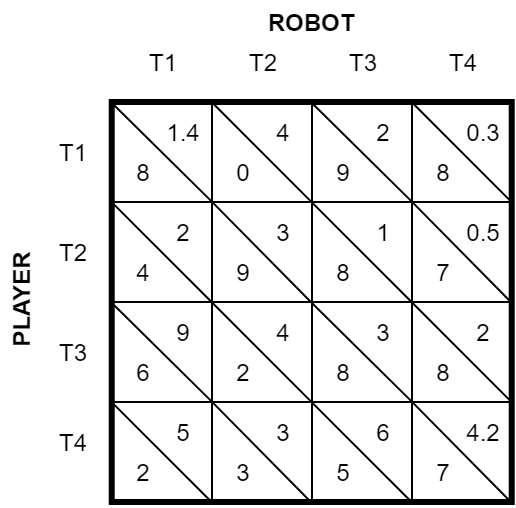
\includegraphics[scale=0.35]{images/06-deception/matrix}
\caption{Example of outcome matrix. The columns represent the  robot's payoff in attacking one of the four towers. The rows represent the player's one. Each element is a couple of values, namely the player's payoff and the robot's payoff.}
\label{fig::matrix}
\end{figure}

As the game is a conflicting game, the two players gain benefit in each other's loss. For this reason, the design of the outcome matrices has been made as described here below: the robot earns a higher payoff when itself and the opponent choose a different target. From a matrix point of view, this is seen as a lower payoff in the diagonal elements, because it represents when the two opponents choose the same action.
On the other hand, the player's outcome matrix is built starting from the fact that the human player earns a higher payoff when his/her choice is the same as the robot's one. For this reason, the values of the diagonal elements must be greater than the non-diagonal ones. 

The approach for calculating the robot's outcome matrix is the following:
\begin{itemize}
\item \textit{Non-diagonal Elements:}\\

\begin{equation}
\gamma_r \cdot \frac{\overrightarrow{t_{robot}}^{(i)}}{\sum_{i}{\overrightarrow{t_{robot}}^{(i)}}} \cdot \frac{\delta(\tau_{i},player)}{\sum{\delta(\tau_{i},player)}}, \forall\tau_{i} \in \mathcal{T}\\ 
\end{equation}
, where $\overrightarrow{t_{robot}}^{(i)}$ refers to the component $i$ on the vector $t_{robot}$.
\item \textit{Diagonal Elements:}
\begin{equation}
\delta(\tau_{i},robot)
\end{equation}
Where $\gamma_r$ is a tuning constant. In the robot's outcome matrix, $\gamma_r$ has been used to weight the values of the non-diagonal values, equation (5), while in the player's matrix, another tuning constant has been used for the diagonal values, equation (8). Tuning the values of the outcome matrices is needed for highlighting the fact that the two players win in two different situations. Giving the right value to $\gamma$ is necessary for having a balanced values for the correspondence-interdependence value.
%TODO It is not clear why a tuning is needed, and hwy the two are the same. 
%[LAURA]: tuning is needed for highlighting the fact that the two players win in different situations or it would best saying that the two win with opposite actions (the robot wants to run 'alone' to the tower while the player prefers to have the robot next to him/her so the robot cannot run and win another tower. Giving the right value to gamma is necessary for having a balanced values for the correspondence-interdependence value. They do not have to be the same
The second term in (5) has been used for giving a weight to the payoff: the more an individual is interested in a given target (supposed that this is a consequence of rational~/~maximizer thinking), the higher the payoff is if the player can obtain it.
The third and last term in (5) expresses how much advantage the player has on the other one.
%TODO This explanation is not clear at all. What are the first, second and third terms? It is hard to understand what they are, both because they are in two different equations (numbers could be used to select them
%[ISTEFF] What about refrasing it in "payoff from equation 5 and 7 can be expressed as a multiplication of three terms: the first one etc...
% The first one, \gamma, is a tuning parameter needed for/because of X;
% Payoffs from equations (5) and (7) can be decomposed in a multiplication of two different terms. The first one is the absolute payoff of a given target (%metacomment what I want to say is that this is the payoff not considering the opponent, which is taken into consideration by the next weight) , as it represents the interest of an individual for it given its own state; the second one expresses the advantage the individual has over the opponent to reach the given target, providing a metric of the reachability of the target considering the opponent.
\end{itemize}

Similarly, the player's outcome is described below:
\begin{itemize}
\item \textit{Non-diagonal Elements:}\\
$\forall\tau \in \mathcal{T}$\\
\begin{equation}
 \frac{\overrightarrow{t_{player}}^{(i)}}{\sum_{i}{\overrightarrow{t_{player}}^{(i)}}} \cdot \frac{\delta(\tau_{i},robot)}{\sum_{i}{\delta(\tau_{i},robot)}}, \, \forall\tau_{i} \in \mathcal{T} 
\end{equation}
\item \textit{Diagonal Elements:}
\begin{equation}
\gamma_p \cdot \frac{1}{\delta(\tau_{i},robot)}
\end{equation}
\end{itemize}

From this, a player's utility is periodically (re)computed and then incorporated into the interdependence-correspondence space~\cite{wagner_acting_2011}.

For our purposes, the \textit{interdependence} dimension represents the correlation between the two players' outcome matrices, while \textit{correspondence} one quantifies how much conflict exists between the two selected actions.

The two values are calculated keeping in mind three concepts: the variation of the robot's outcome matrix resulting from its own decisions; the variation of the player's outcome matrix resulting from the partner's decisions; the variance in outcome matrix resulting from both, joint, interactive decisions.

The calculations for interdependence are made as in algorithm~\ref{alg:interdependence}, where $\alpha \in[-1;0]$, and $\Delta$ expresses the maximum variation the player can obtain on the robot's outcome matrix. The variable \textit{total} expresses the range used for normalization, and $n(\mathcal{T})$ the number of towers.

\begin{algorithm}[h]
\SetAlgoLined
\SetKwInOut{Input}{input}\SetKwInOut{Output}{output}
\Input{Robot's outcome matrix}
\Output{Float value}
\BlankLine
\For{$i \in range(1,n(\mathcal{T}))$ }{
$\Delta_{outcomes} = | max_{outcome(:,i)} - min_{outcome(:,i)} | $ \\
$total = max_{outcome(:,i)} + min_{outcome(:,i)} $\\
$\alpha \mathrel{{+}{=}} \frac{\overrightarrow{t_{robot}}^{(i)}}{\sum_{i}{\overrightarrow{t_{robot}}^{(i)}}} \cdot \frac{\Delta}{total}$
}
\caption{Interdependence algorithm}
\label{alg:interdependence}
\end{algorithm}

The procedure to calculate the correspondence value is defined in algorithm~\ref{alg:correspondence}, where $\beta \in[0;1]$.
\begin{algorithm}[h]
\SetAlgoLined
\SetKwInOut{Input}{input}\SetKwInOut{Output}{output}
\Input{Outcome matrices}
\Output{Float value}
\BlankLine
\textit{Avg(outcome $\forall$ Robot's action)}\\
\textit{Avg(outcome $\forall$ Player's action)}\\

\For{$i \in range(1,n(\mathcal{T}))$}{
\textit{amr = tower index that maximizes robot's outcome} \\
\textit{amp = tower index that maximizes player's outcome} \\
$\Delta_{robot} = outcome_{robot}(amr,i) - outcome_{robot}(amp,i) $ \\
$\Delta_{player} = outcome_{player}(amr,i) - outcome_{player}(amp,i) $ \\
$total_{robot} = outcome_{robot}(amr,i) + outcome_{robot}(amp,i)$ \\
$total_{player} = outcome_{player}(amr,i) + outcome_{player}(amp,i)$ \\
$\beta \mathrel{{+}{=}} \frac{1}{2} \cdot \frac{Avg_{robot}}{\sum{Avg_{robot}}} \cdot \frac{\Delta_{robot}}{total_{robot}} \cdot \frac{\Delta_{player}}{total_{player}}$
}
\For{$i \in range(1,n(\mathcal{T}))$}{
\textit{amr = tower index that maximizes robot's outcome} \\
\textit{amp = tower index that maximizes player's outcome} \\
$\Delta_{robot} = outcome_{robot}(i,amr) - outcome_{robot}(i,amp) $ \\
$\Delta_{player} = outcome_{player}(i,amr) - outcome_{player}(i,amp) $ \\
$total_{robot} = outcome_{robot}(i,amr) + outcome_{robot}(i,amp)$ \\
$total_{player} = outcome_{player}(i,amr) + outcome_{player}(i,amp)$ \\
$\beta \mathrel{{+}{=}} \frac{1}{2} \cdot \frac{Avg_{player}}{\sum{Avg_{player}}} \cdot \frac{\Delta_{robot}}{total_{robot}} \cdot \frac{\Delta_{player}}{total_{player}}$
}
\caption{Correspondence algorithm}
\label{alg:correspondence}
\end{algorithm}
The procedure works by going through every action the robot and the player can take. For example, if the robot decides to take action 1 (go to tower 1), it temporally ignores all the other columns of the robot's outcome matrix and checks what are the indexes that maximize the robot's outcome and the player's one. It then calculates the difference between the outcomes using the two indexes (for both robot and player); a negative $\Delta$ means for the subject that the situation is a conflict (the values of the outcome matrix are positive). The variations are normalized and multiplied by each other and then multiplied by a factor that expresses how likely the action would be taken (if an action will not be chosen, $\beta$ will have a lower impact). Similarly, the same procedure is done w.r.t. the player's actions.

In \textit{Figure~\ref{fig::interdependece}} the correspondence and interdependence space distributions are represented. By making a discretization of the playground into a grid and placing the robot at (4,5), while varying the  player's position on every other coordinate, it is possible to notice that the diagonal that leads to the towers has a higher value of dependency and conflict.

The mapping of the situation to the space shows when deception may be needed. Once an extremely dependent and conflicting situation is detected, deception is triggered.

\begin{figure*}[t]
\centering
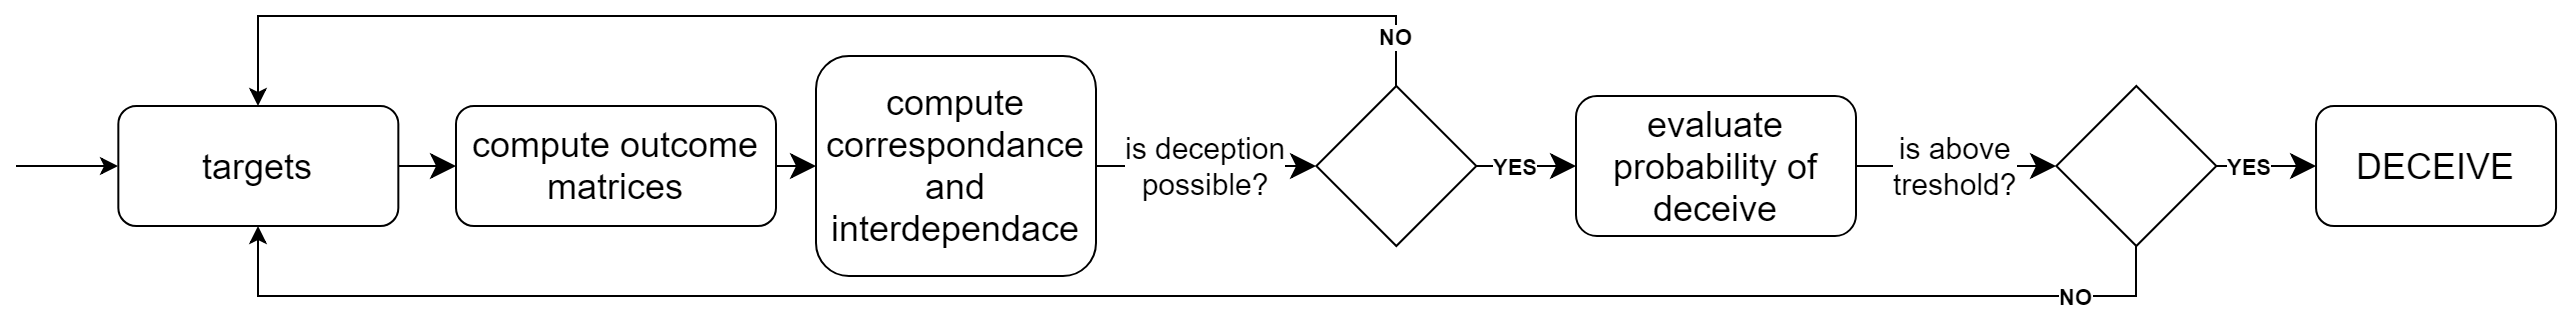
\includegraphics[width=\textwidth]{images/06-deception/flowchart}
\caption{The procedure to select deception}
\label{fig:flowchart}
\end{figure*}

Once deception is warranted, the algorithm calculates the fake target to be communicated to the player. The fake target is chosen in the following steps: after the real target is established, the robot calculates two actions that would give the robot the highest rewards and, finally, it calculates which of the two maximizes the player's payoff. This last step expresses the incentive for the player to approach the fake target. The algorithm is detailed in Figure~\ref{fig:flowchart}.

\begin{figure}[H]
\centering
  \begin{subfigure}[t]{0.49\columnwidth}
  \centering
    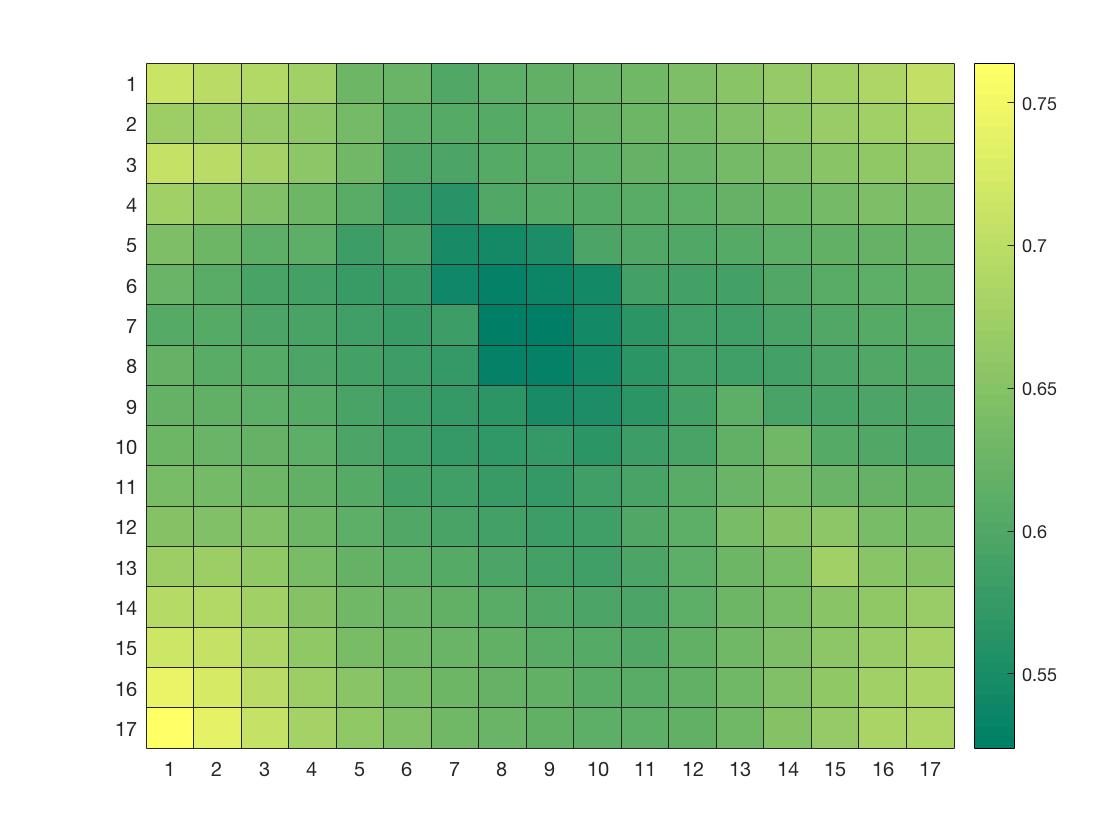
\includegraphics[width=\linewidth]{images/06-deception/interdependence.jpg}
    \caption{}
    \label{fig:interdipendence}
  \end{subfigure}
  %\hspace{0.01\columnwidth}
  \begin{subfigure}[t]{0.49\columnwidth}
  \centering
    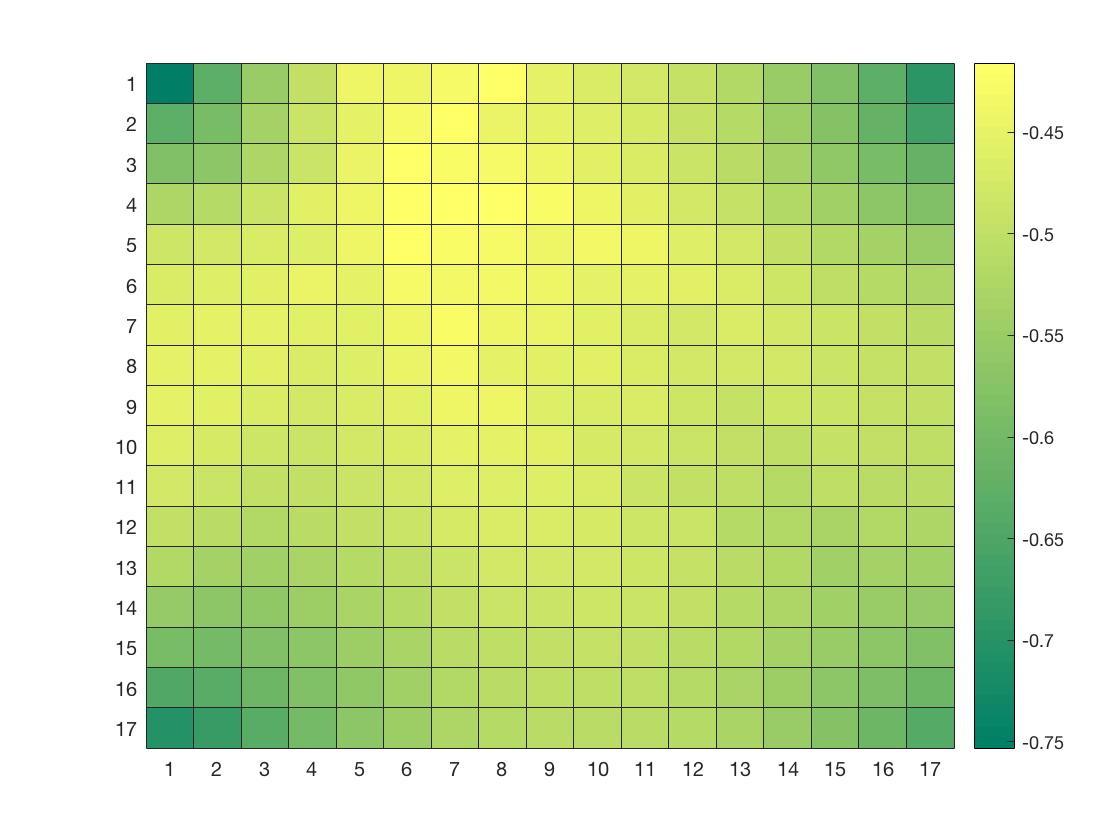
\includegraphics[width=\linewidth]{images/06-deception/correspondence.jpg}
    \caption{}
    \label{fig:correspondence}
  \end{subfigure}
  \caption{Space distribution of the correspondence and interdependence when the robot is placed in (4,5). (a) Interdependence space distribution; darker cells correspond to lower interdependence. (b) Correspondence space distribution; brighter cells indicate lower correspondence.}
  \label{fig::interdependece}
\end{figure}

\subsection{Communicating false goals}
Having presented how to trigger deception, in this section we describe means of effectively using deceptive behavior by communicating false goals, i.e., false attempts to knock down towers. We begin by describing the two methods used.
\subsubsection{Static trajectory approach}
In this first method the trajectories are established a priori. It means that once the navigation node receives the fake and real target information, it calculates, based on the actual position of the robot, the series of points the robot needs to follow in order to communicate the deception.
The algorithm can choose between two different types of trajectories. The first one is activated when the robot is halfway through the fixed frame of localization (map, on the ROS jargon). The robot will then move forward without letting the player know which tower is going to be hit, leaving 50\% of chance of guessing. Only when ``close'', within a predefined threshold, to the midpoint of a virtual line connecting the two towers (true and fake target, respectively), the robot changes trajectory towards the true target.

The second type of deception will try to communicate from the beginning the fake target in order to let the player run and stay to a particular tower, and in this way take spatial advantage when trying to knock down the real target. A pictorially description of such trajectories is shown in Figure~\ref{fig::trajectoryStatic}.

The trajectories are implemented by deciding a series of points to be followed. Those points are spatially distributed along the desired trajectory (Figure \ref{fig::trajectoryStatic}).
% In the first type of deception, the middle point between the two targets is calculated, then three points are extracted in the segment between the robot's position and the middle point. Once reached the third point, the robot changes direction and goes to the real target. %TODO This is different from what shown in the figure.
% Similarly happens in the other type of deception where the subsequent points are calculated between the robot and the fake target, once reached the second or third point of this sequence, the robot changes direction and goes to the real target.

In the present proposal, deception is considered as a complete 'path' that starts when the robot receives the deception information (true and fake tower) and lasts until the robot hits the tower. Since no look-ahead for determining the player position in the future has been considered, it can happen that the player understands the deception and/or the player is really reactive and blocks the robot, so that it would be difficult to finish the deception procedure coherently.
For this reason, the algorithm calculates the time required for successfully making the deception and, every time something goes wrong (for example, the player blocks the robot), the estimated time expires and the deception procedure is aborted. Once it happens, the normal procedure starts again to compute a regular target, until a new need for deception is detected.
\begin{figure}[H]
\centering
  \begin{subfigure}[t]{0.45\columnwidth}
  \centering
    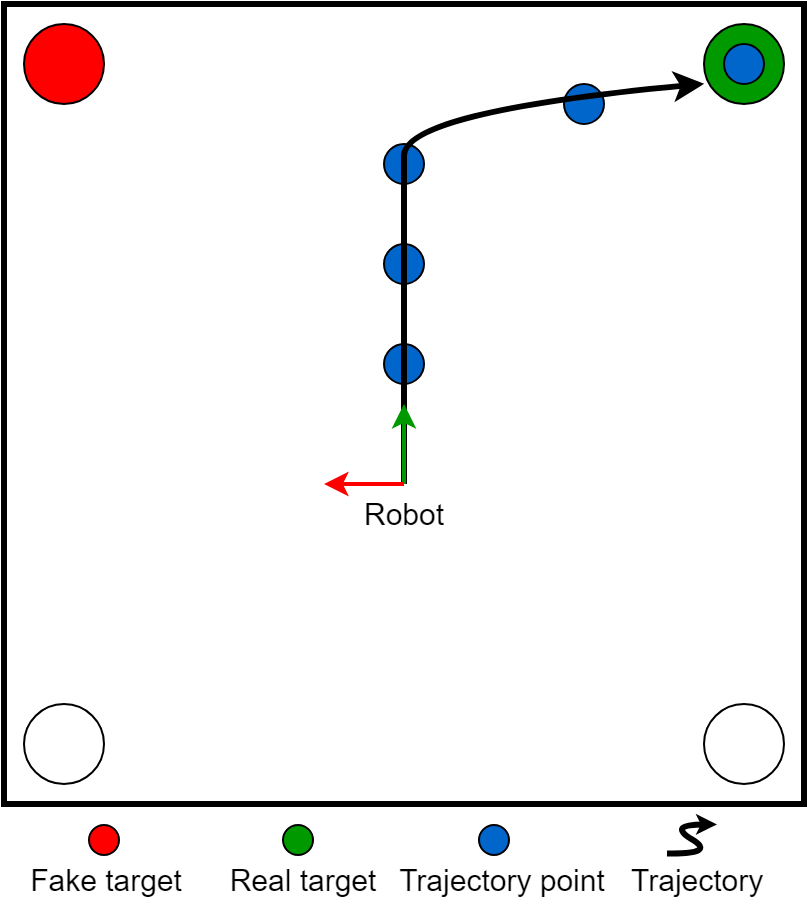
\includegraphics[width=\linewidth]{images/06-deception/trajectoryLaura}
    \caption{Moving forward and then changing the direction.}
    \label{fig:1}
  \end{subfigure}
  \hspace{0.01\columnwidth}
  \begin{subfigure}[t]{0.45\columnwidth}
  \centering
    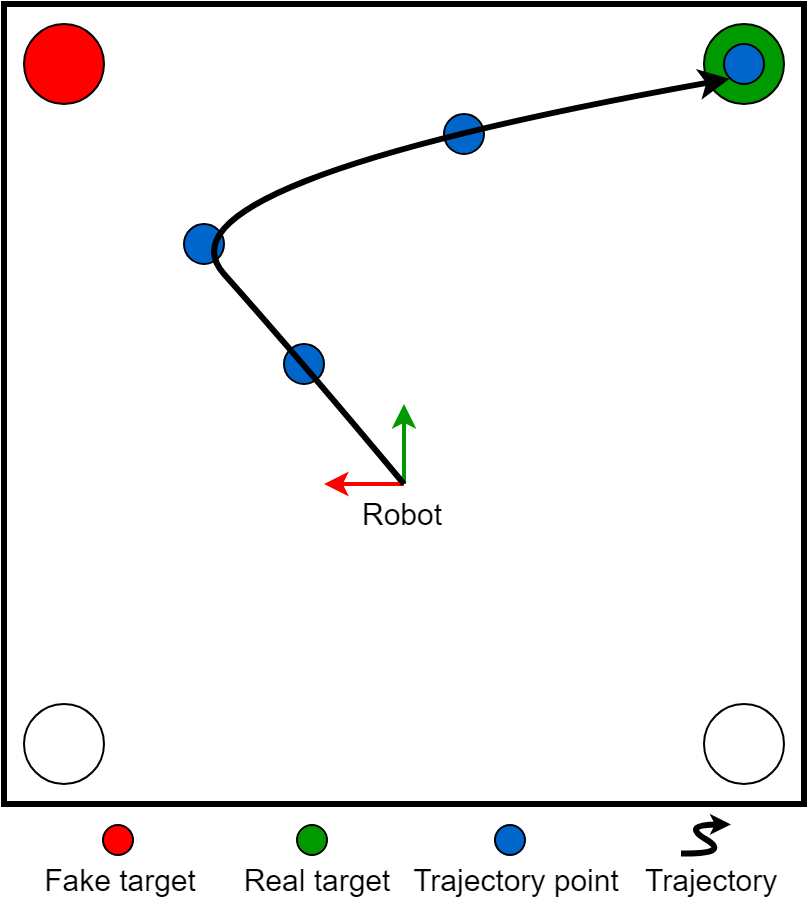
\includegraphics[width=\linewidth]{images/06-deception/trajectoryLaura2}
    \caption{Moving toward the false target and then changing direction.}
    \label{fig:2}
  \end{subfigure}
  \caption{The two types of deception when using the static trajectory approach.}
  \label{fig::trajectoryStatic}
\end{figure}

\subsubsection{Dynamic steering behavior approach}
The second approach we propose in order to implement a deceiving trajectory is based on steering behaviors~\cite{reynolds_steering_1999}. The paper by Reynolds proposes a force-based approach to guide an actor in a life-like and improvisational manner. Given a target, it will generate a force, either attractive or repulsive, based on its position with respect to the robot: by applying this force on the robot, it will be driven either towards or away from the target following a smooth path.

Being our robot holonomic, it has been represented as a point mass to calculate the results of the application of the forces generated by the steering behavior. This approach gives us the possibility to dynamically change the robot response to forces by changing the kinematic properties of our representation during the calculation process.

Instead of planning the complete trajectory, only the point where we want to change the motion parameters of the robot and reveal the true target is computed and set as a temporary target. The steering behavior framework drives the robot to reach this target following a slightly different trajectory each time based on its initial velocity and position.

In order to follow a deceptive trajectory as previously described, the dexterity of the robot is dynamically increased when revealing its real target: once the temporary target is reached the virtual mass of the robot is lowered and a higher force is allowed to be applied to it, along with a slight increase on its maximum velocity: then the target to be reached is set to the real target. This procedure generates a sharp turn and an acceleration of the robot towards the real goal. A visualization of the parameter change effect can be seen in Figure~\ref{fig::trajectorySteering}. 

Given this framework, we wanted to investigate whether such change of motion pattern helps the player to realize that the intention carried out by the robot had been to deceive and whether diversity of trajectories increases the appeal of the game by making the robot movements less predictable.

\begin{figure}[htbp]
\centering
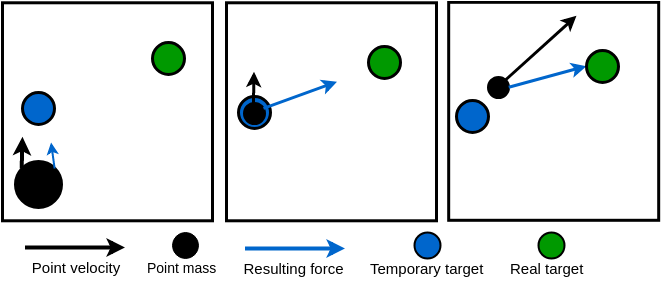
\includegraphics[scale=0.33]{images/06-deception/parameterUpdate}
\caption{Update in vehicle parameters and target will produce an increment in robot velocity as well as a smooth bend in the real target direction: on the left we're approaching the temporary target; on the center we change the parameters as we reach the temporary target; on the right we move towards the real target with new parameters}
\label{fig::trajectorySteering}
\end{figure}

%[EWERTON] --> \subsubsection{A machine learning approach} {\color{red} This is going to be used in a follow up project. What about some Journal? YES Social Robotics}

\section{Validation}
\label{S:Validation}
In this section, we describe the acceptability of our strategy within the mentioned interactive scenario. We first present the experimental setup, stating the hypothesis and the use of a post-match survey for evaluating them. The analysis and related discussion follow next. 

%TODO The following sentence was probably left here in editing -> Results from self-report responses to questionnaires filled-up by the participant after each game match.

\subsection{Experimental setup}
\subsubsection{Hypotheses}

\paragraph{H1} The subjects enjoy the game.
\paragraph{H2} The subjects consider the robot as a rational agent, aiming at winning since it is participating to a competitive game.
\paragraph{H3} The two trajectory approaches are both able to create a recognizable level of deception. 
\paragraph{H4} The dynamic steering approach appeals more than the static one.

\subsubsection{Factors}
During our experiments we have kept the parameters that control the general game difficulty discrete such as: maximum speed and maximum acceleration. It was part of our project decision to limit the effect of such variables in this study, while, at the same time, improve safety (since a possible collision against a fast robot is dangerous) and reduce the risk of mechanical problems, since frequent, abrupt acceleration/deceleration might damage the wheel-motor joints.

Speed and acceleration values define two different levels: easy (speed = $0.5m/sec$ and acceleration = $0.1m/sec^2$) and medium (speed = $0.7m/sec$ and acceleration = $0.5m/sec^2$).

However, during experimentation we have noticed that the difficulty level set to easy turned out to be too slow. Therefore, in order to maintain consistency in the analysis while also improving fun we have decided to keep the difficulty fixed at the medium level for all the subjects.

In summary, the only varying factors were the approaches for communicating false goals, i.e., the static trajectory and dynamic steering behavior.

\subsection{Post-Match Survey}

After every match, a questionnaire was administered to each player. It included few questions about the subject (including age and gender) and eleven questions about the game. In this paper, we present results about only four of them, relevant to evaluate the specific hypotheses.

\subsection{Participants}
We recruited 91 participants among the visitors of a science fair. %in Milan held between September 28th and 29th, 2018. 
Most of the experiments were conducted with children, spanning from 5 to 15 years old, while some adults from 16 to 54 years old also accepted to play the game. The distribution of subjects is reported in table~\ref{table::subjectDistribution}. Data collection was performed with subjects being sampled on different times of the day in the attempt to randomize the subjects as best as possible. 

\begin{table}[htbp]
\caption{Gender distribution during the experiments with the static and dynamic trajectory approach.}
\begin{center}
\begin{tabular}{|c|c|c|c|c|}
\hline
\multirow{ 2}{*}{\textbf{Trajectory}} & \textbf{Subject}&\multicolumn{2}{|c|}{\textbf{Gender}} & \multirow{ 2}{*}{\textbf{\textit{Total}}} \\
\cline{3-4}
 & \textbf{Age} & \textbf{\textit{Male}}& \textbf{\textit{Female}} &  \\
\hline
\multirow{ 2}{*}{\textbf{Static}} & Children $(<16)$ & 29 & 19 & 48 \\\cline{2-5}
& Adults $(\geq 16)$ & 6 & 7 & 13 \\
\hline
\hline
\multirow{ 2}{*}{\textbf{Dynamic}} & Children $(<16)$ & 12 & 16 & 28 \\\cline{2-5}
& Adults $(\geq 16)$ & 2 & 0 & 2 \\
\hline
\end{tabular}
\label{table::subjectDistribution}
\end{center}
\end{table}

\begin{figure*}[t]
\centering
  \begin{subfigure}[t]{0.49\columnwidth}
    \centering
    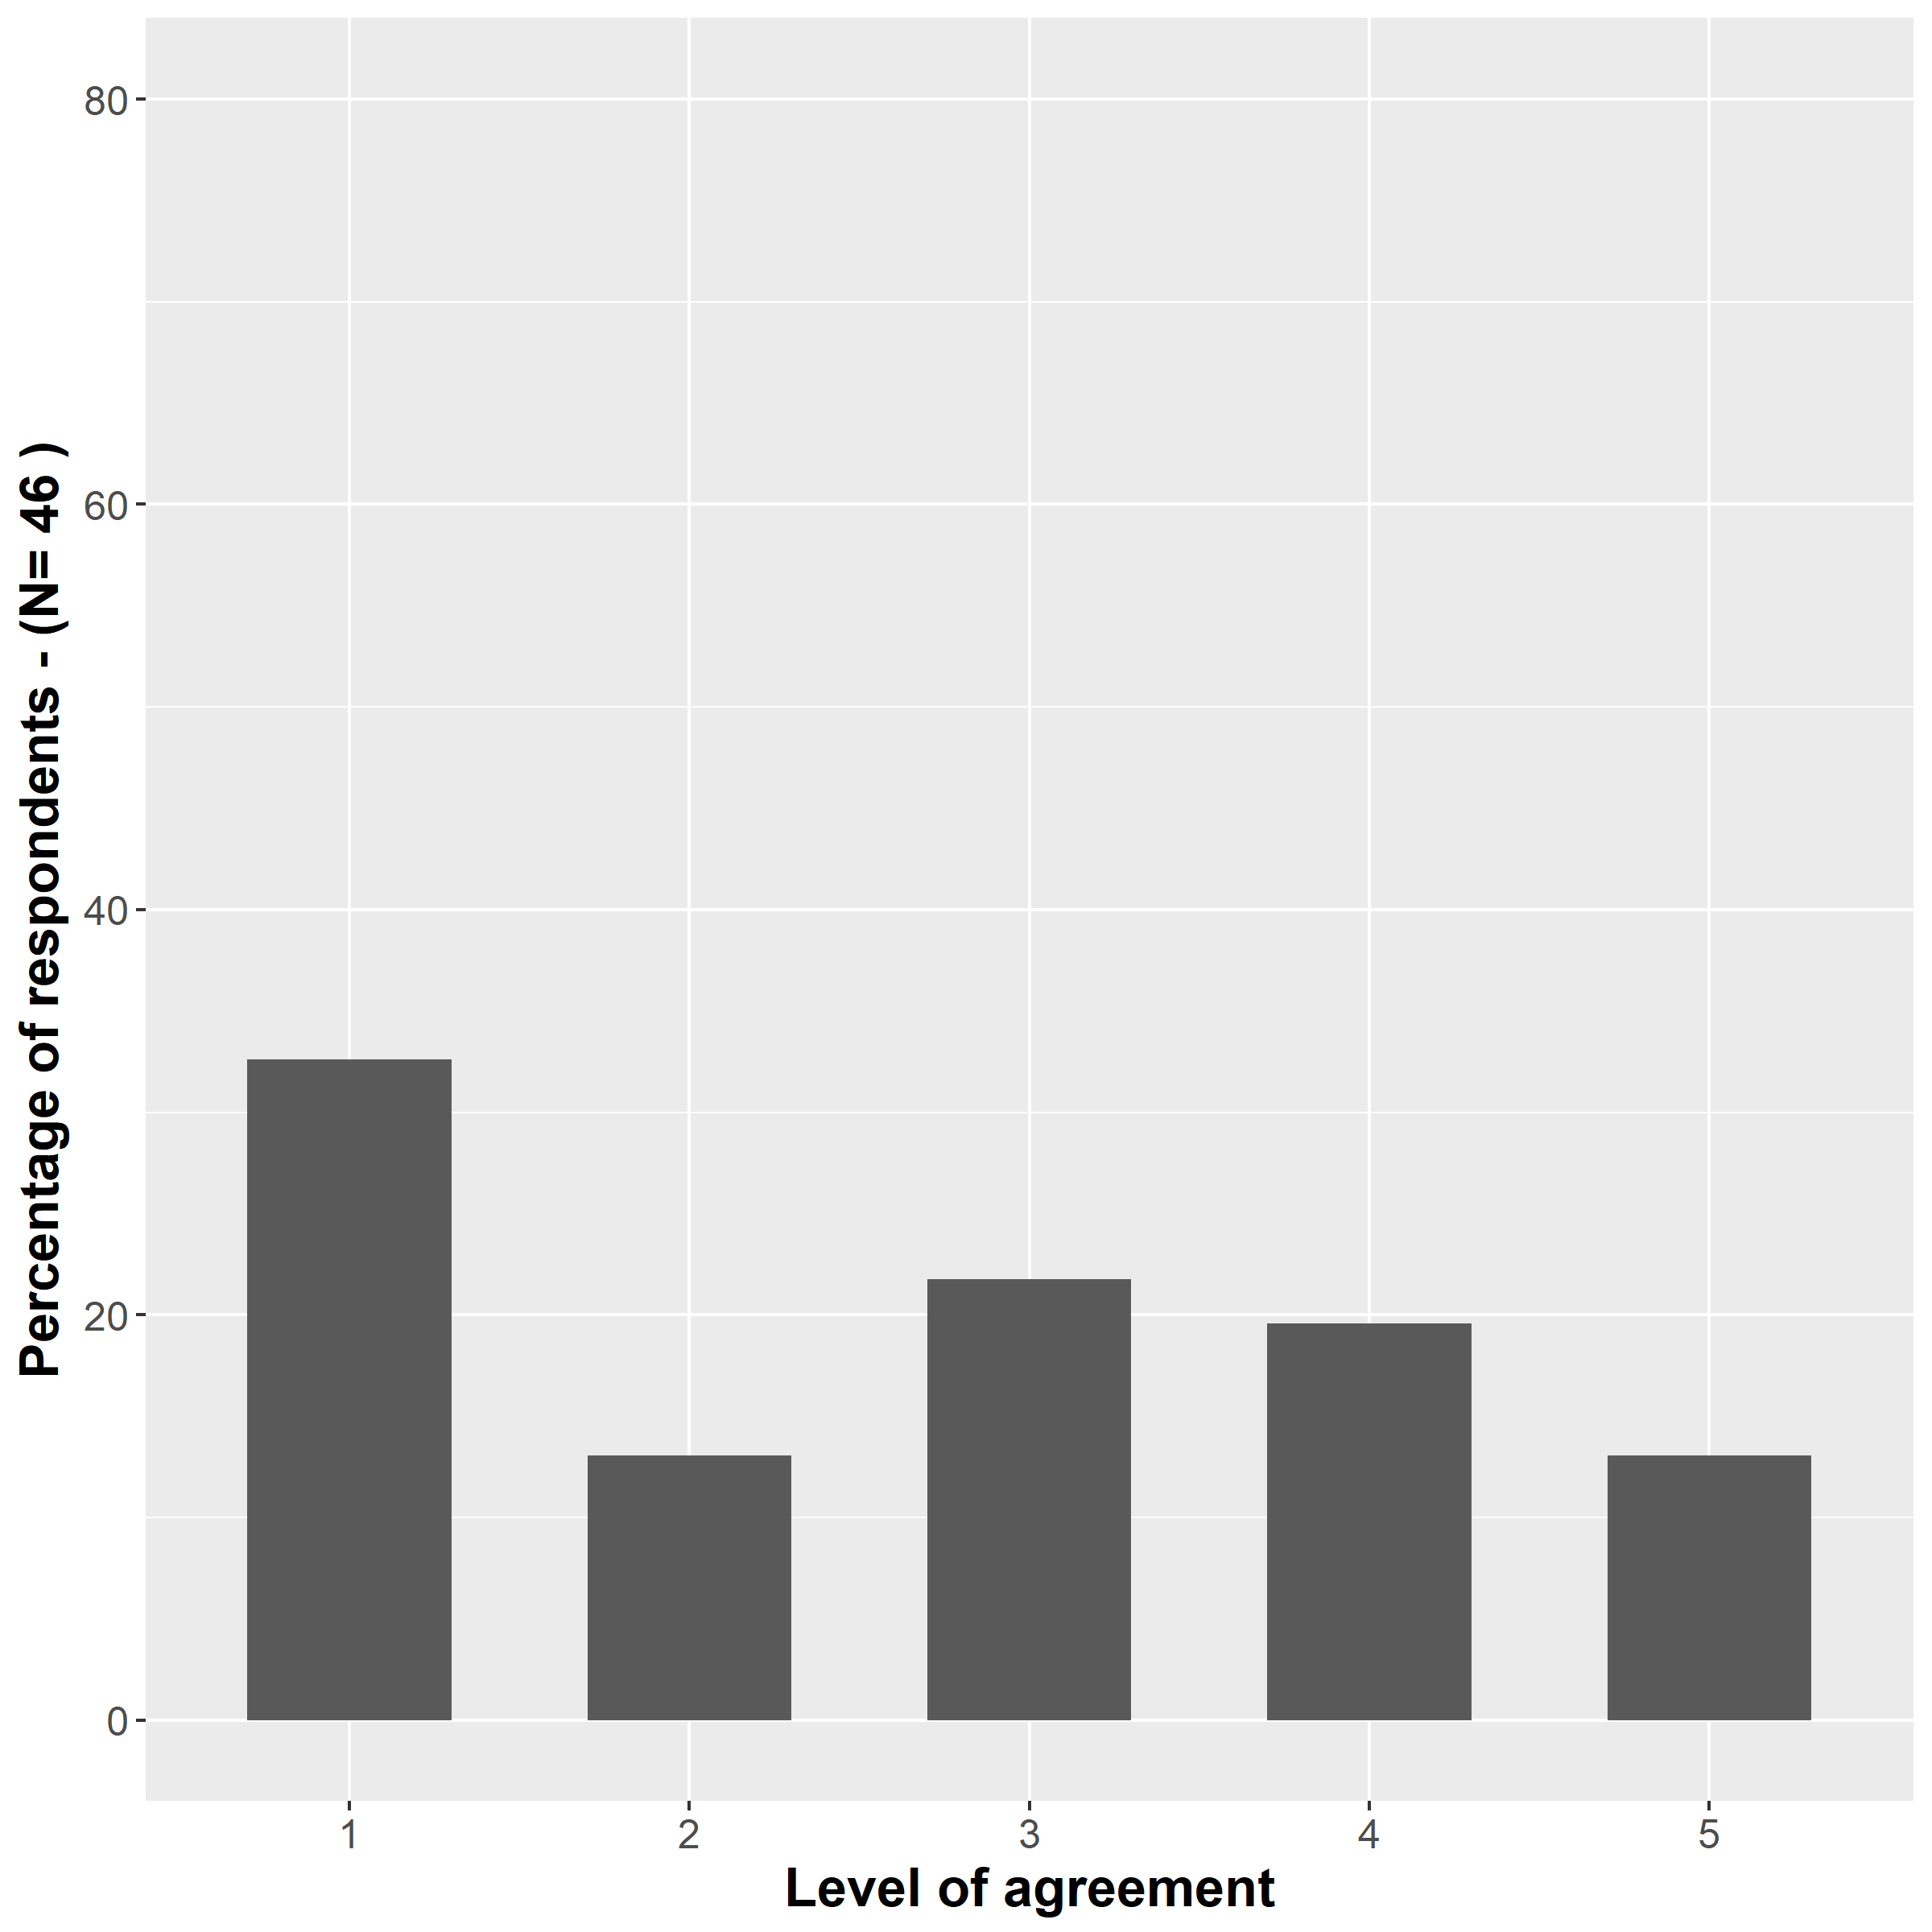
\includegraphics[width=\linewidth]{images/06-deception/staticTooShortYoung}
    \caption{Too short - children.}
    \label{fig::staticTooShortYoung}
  \end{subfigure}
  \hspace{0.01\columnwidth}
  \begin{subfigure}[t]{0.49\columnwidth}
    \centering
    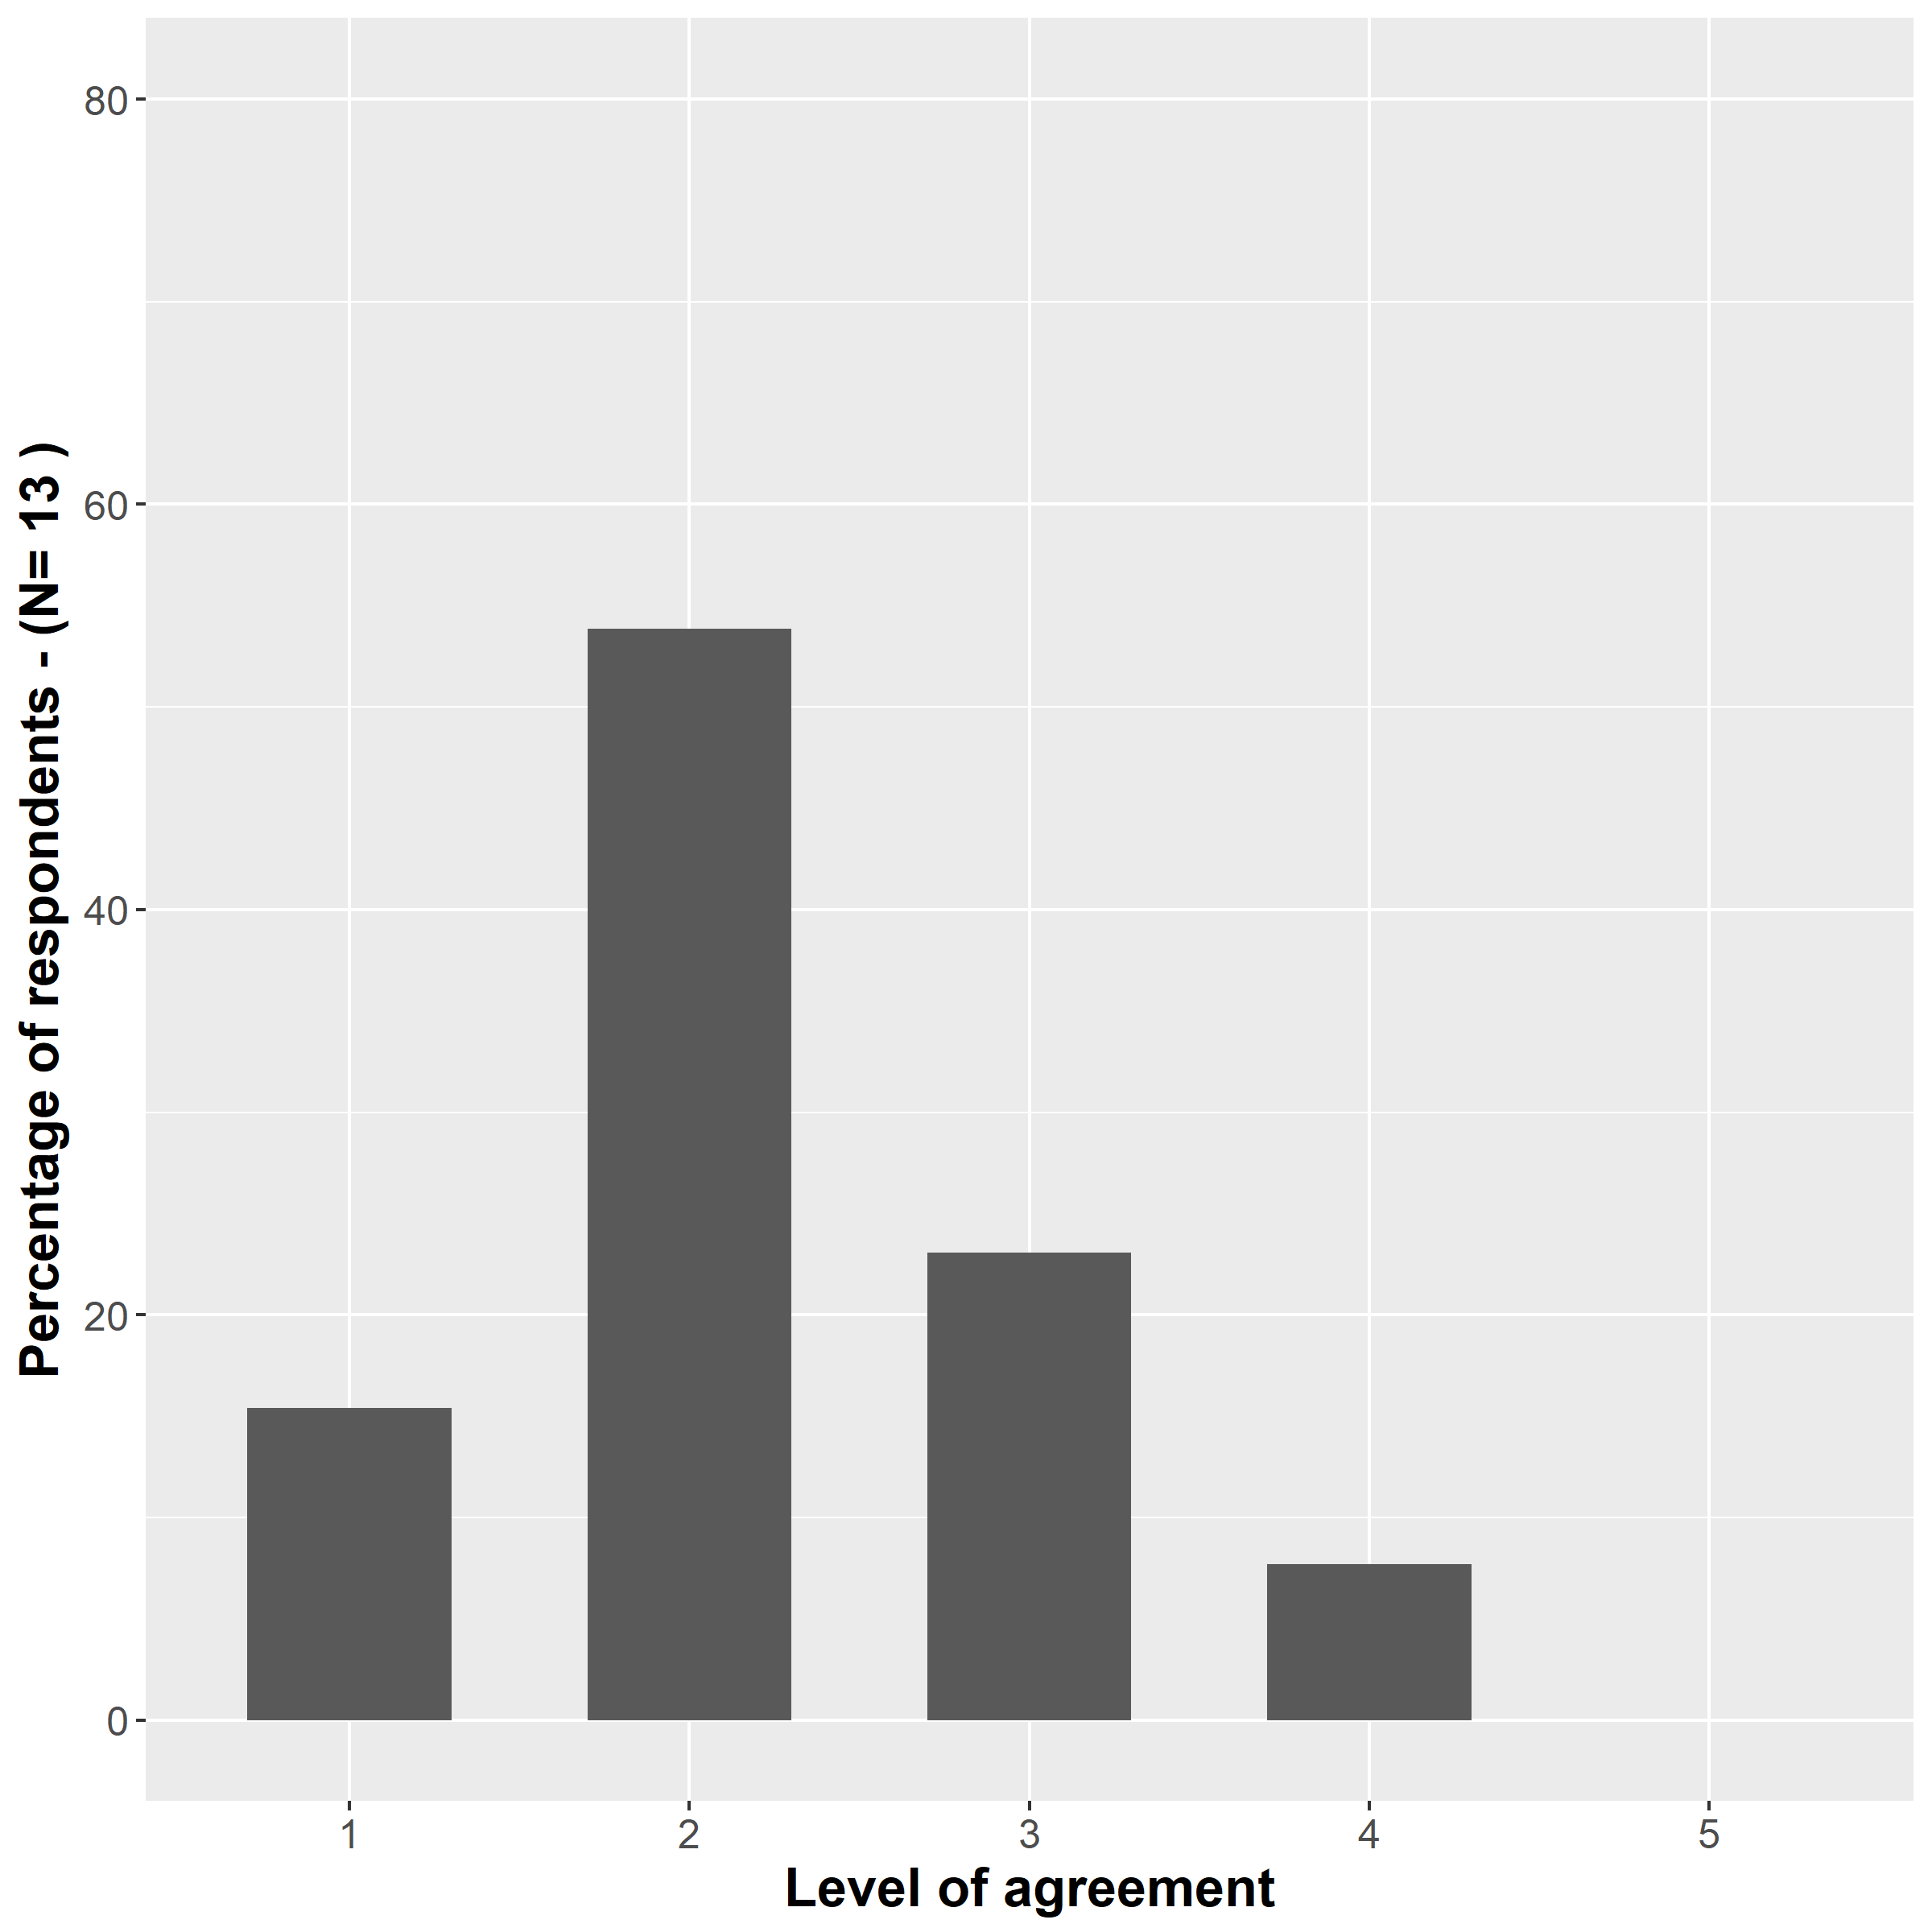
\includegraphics[width=\linewidth]{images/06-deception/staticTooShortAdults}
    \caption{Too short - adults.}
    \label{fig::staticTooShortAdults}
  \end{subfigure}
  %\hspace{0.01\columnwidth}
  \begin{subfigure}[t]{0.49\columnwidth}
  \centering
    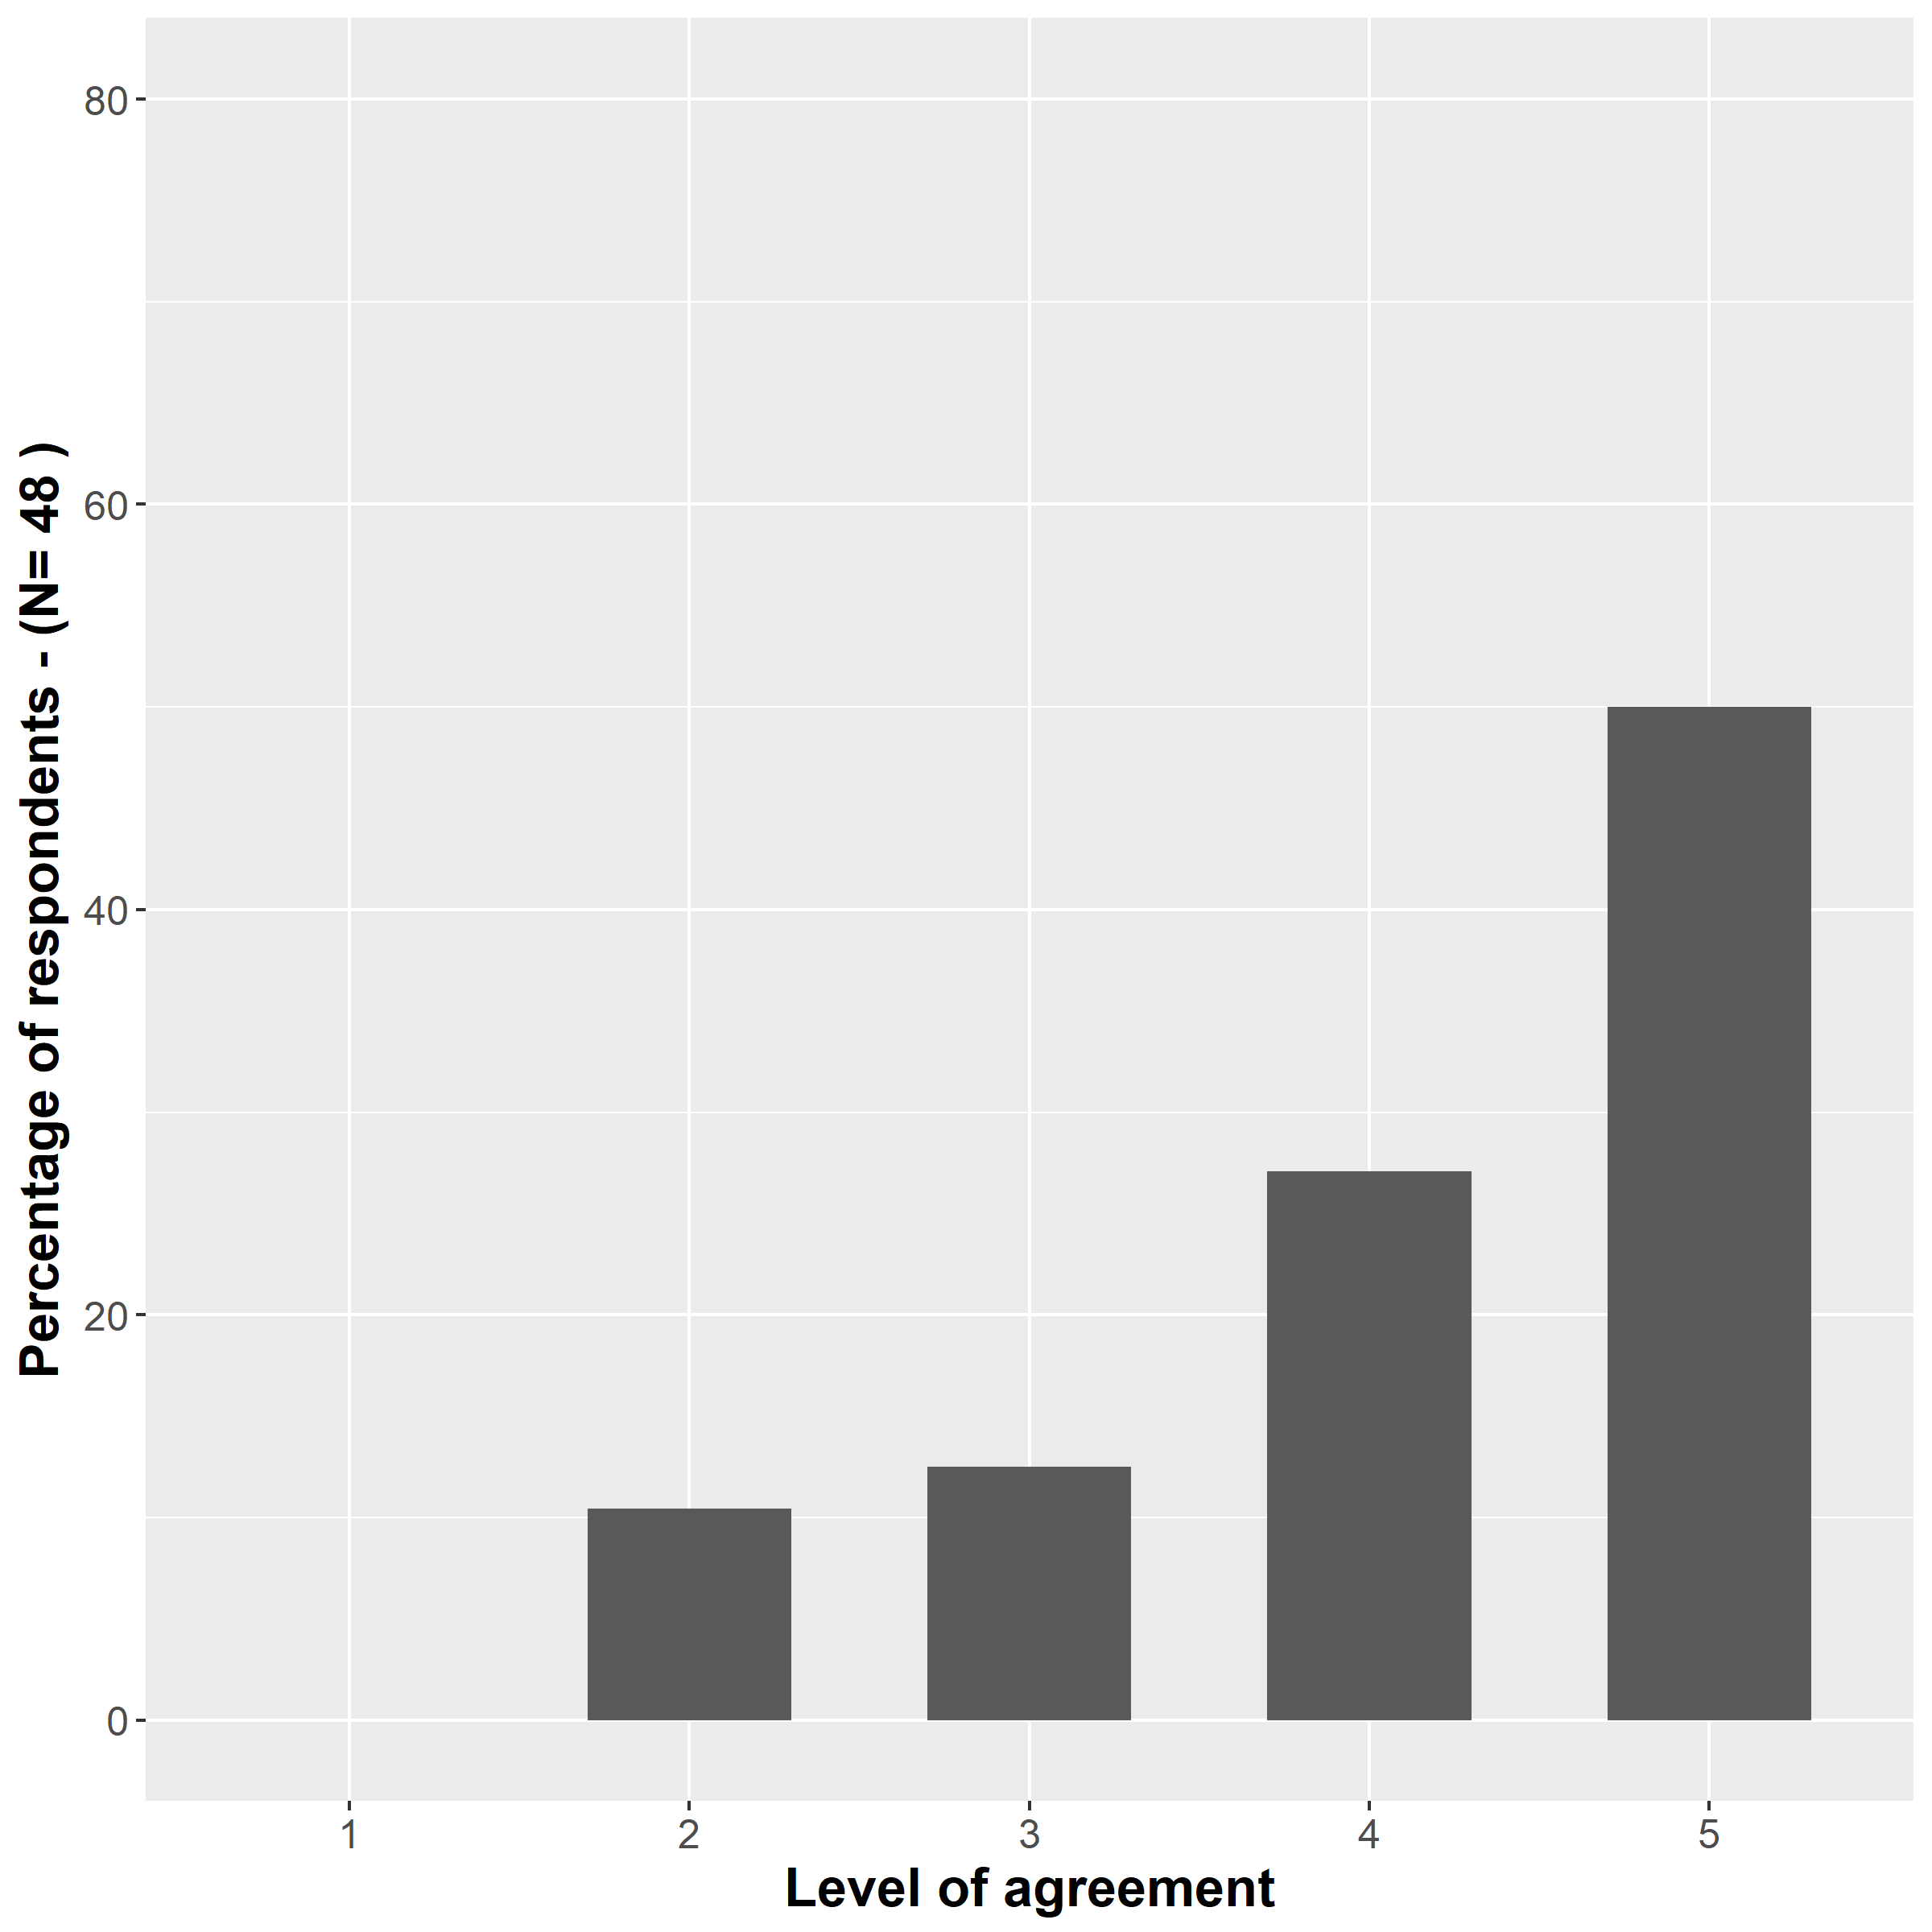
\includegraphics[width=\linewidth]{images/06-deception/staticWinYoung}
    \caption{Robot wants win - children.}
    \label{fig::staticWinYoung}
  \end{subfigure} 
  %\hspace{0.01\columnwidth} 
  \begin{subfigure}[t]{0.49\columnwidth}
    \centering
    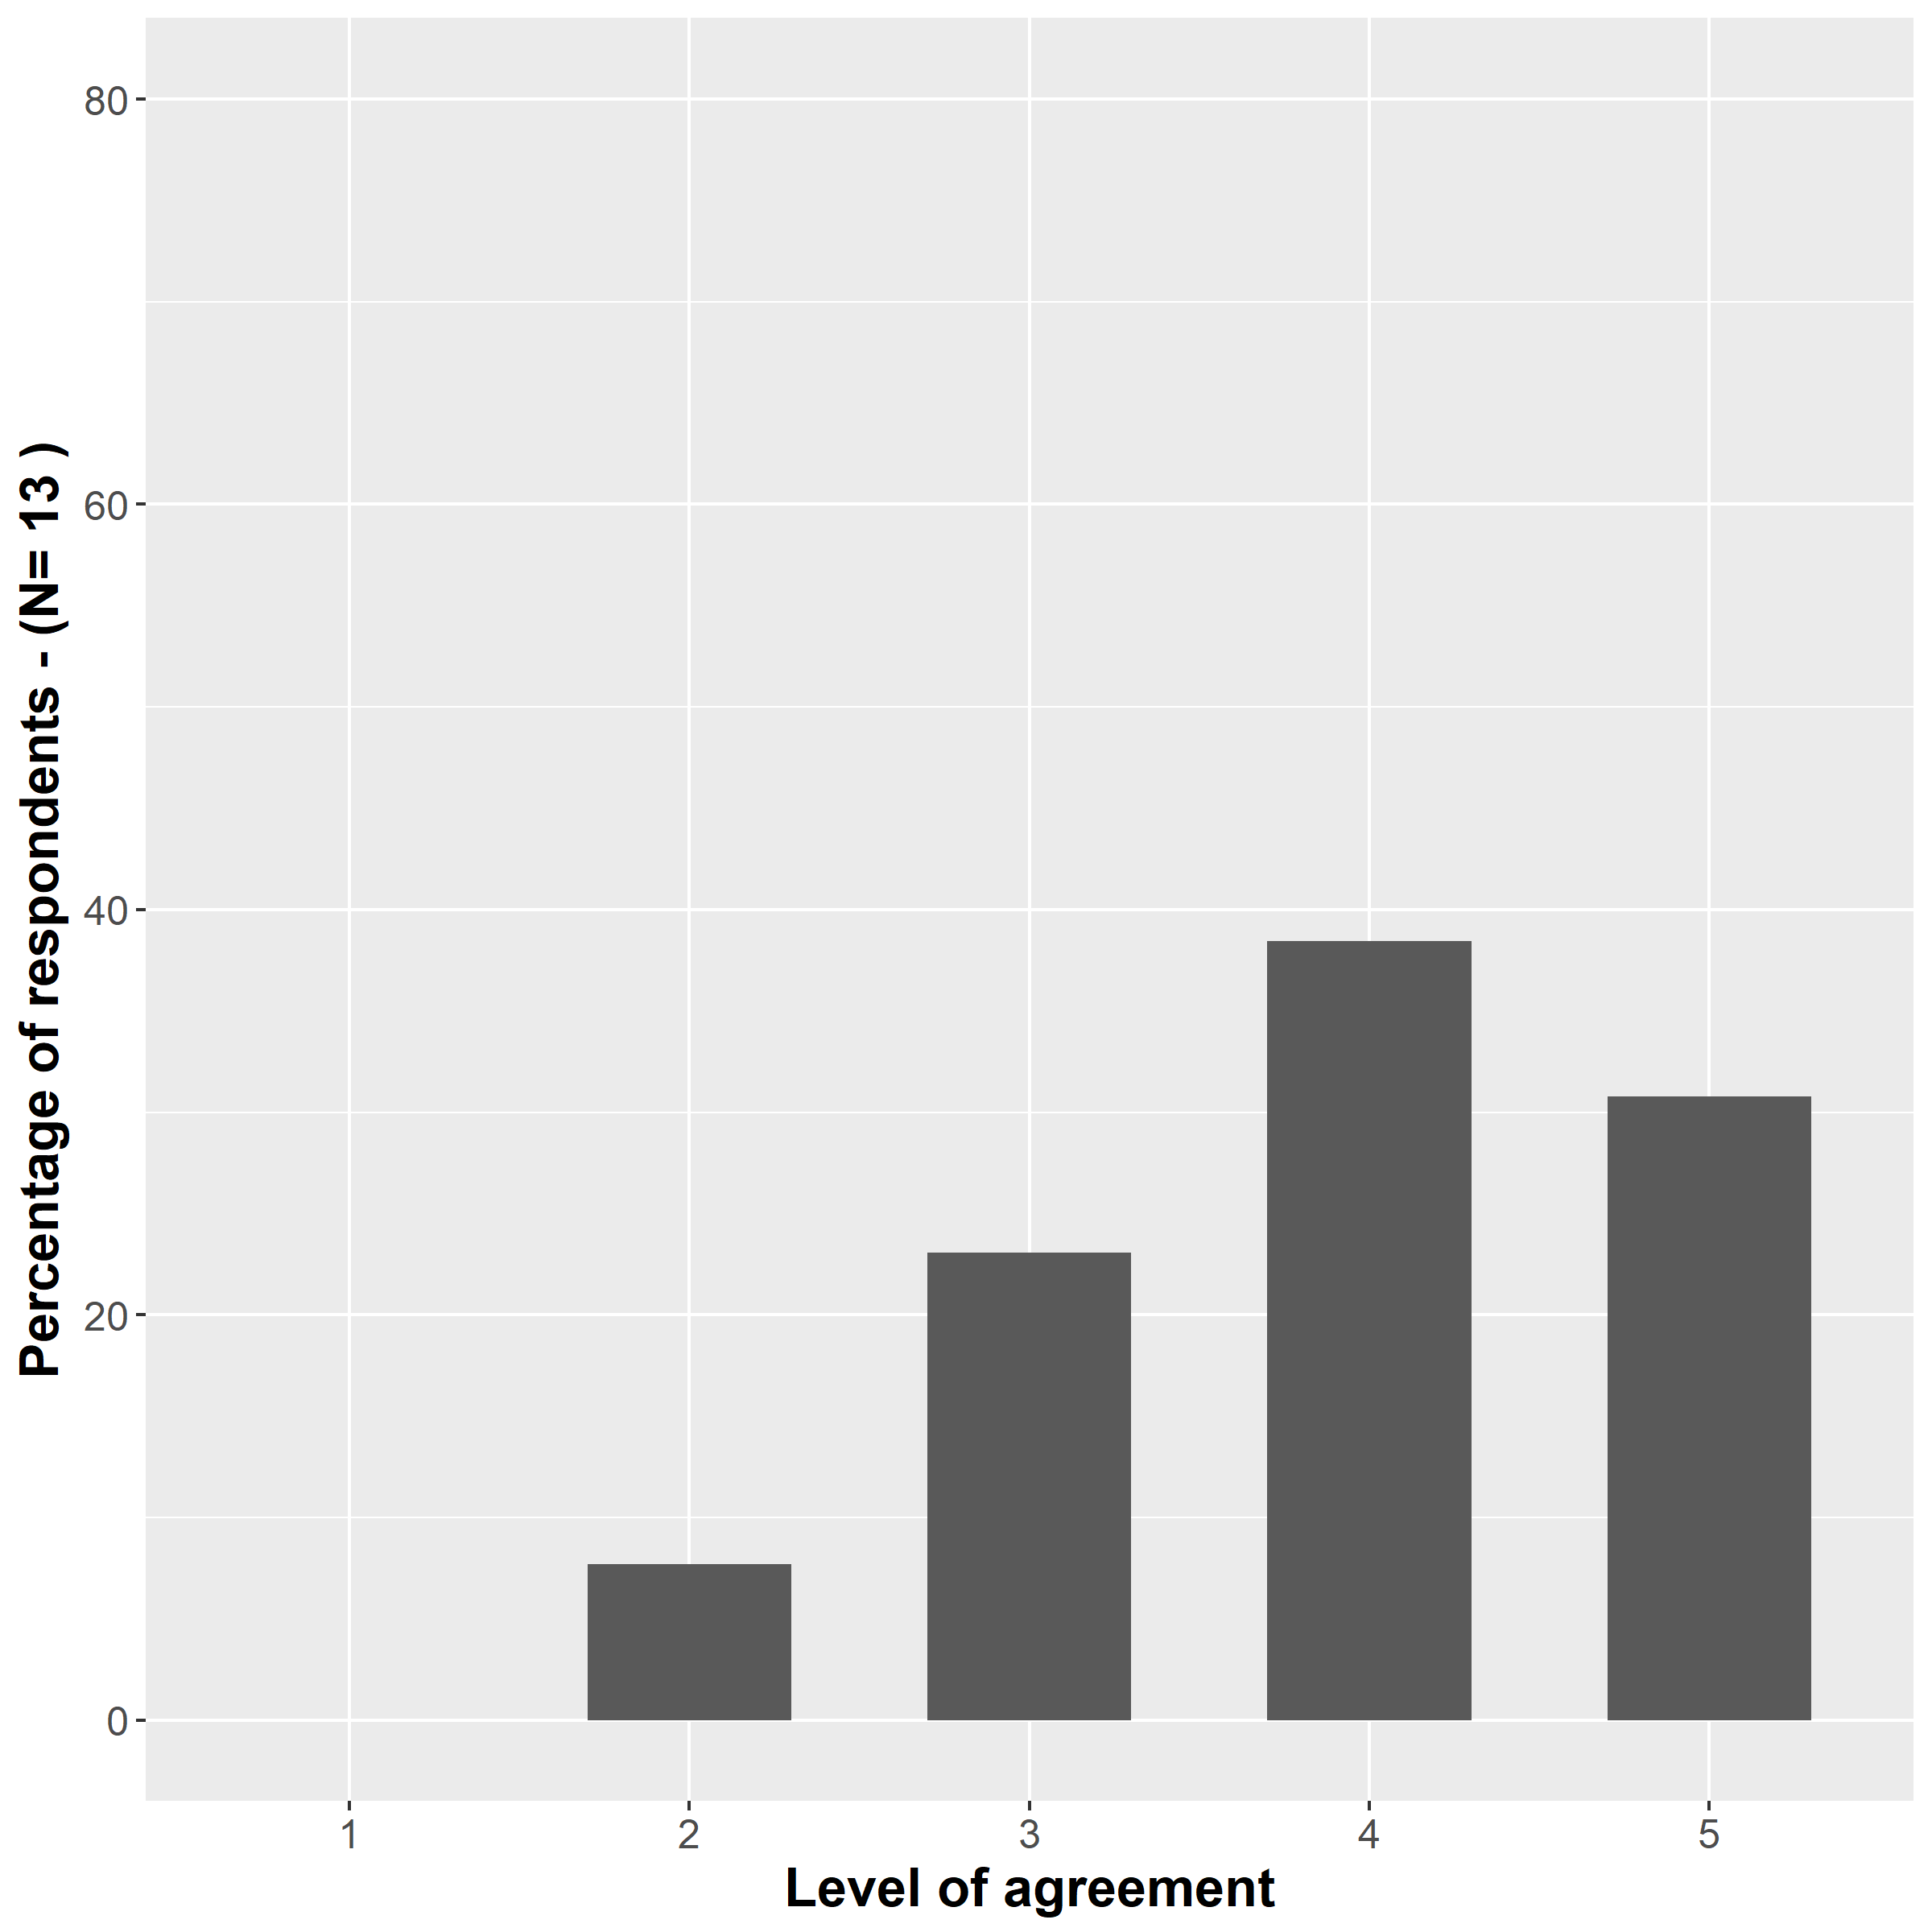
\includegraphics[width=\linewidth]{images/06-deception/staticWinAdults}
    \caption{Robot wants win - adults.}
    \label{fig::staticWinAdults}
  \end{subfigure}
  %\hspace{0.1\columnwidth}
  \begin{subfigure}[t]{0.49\columnwidth}
  \centering
    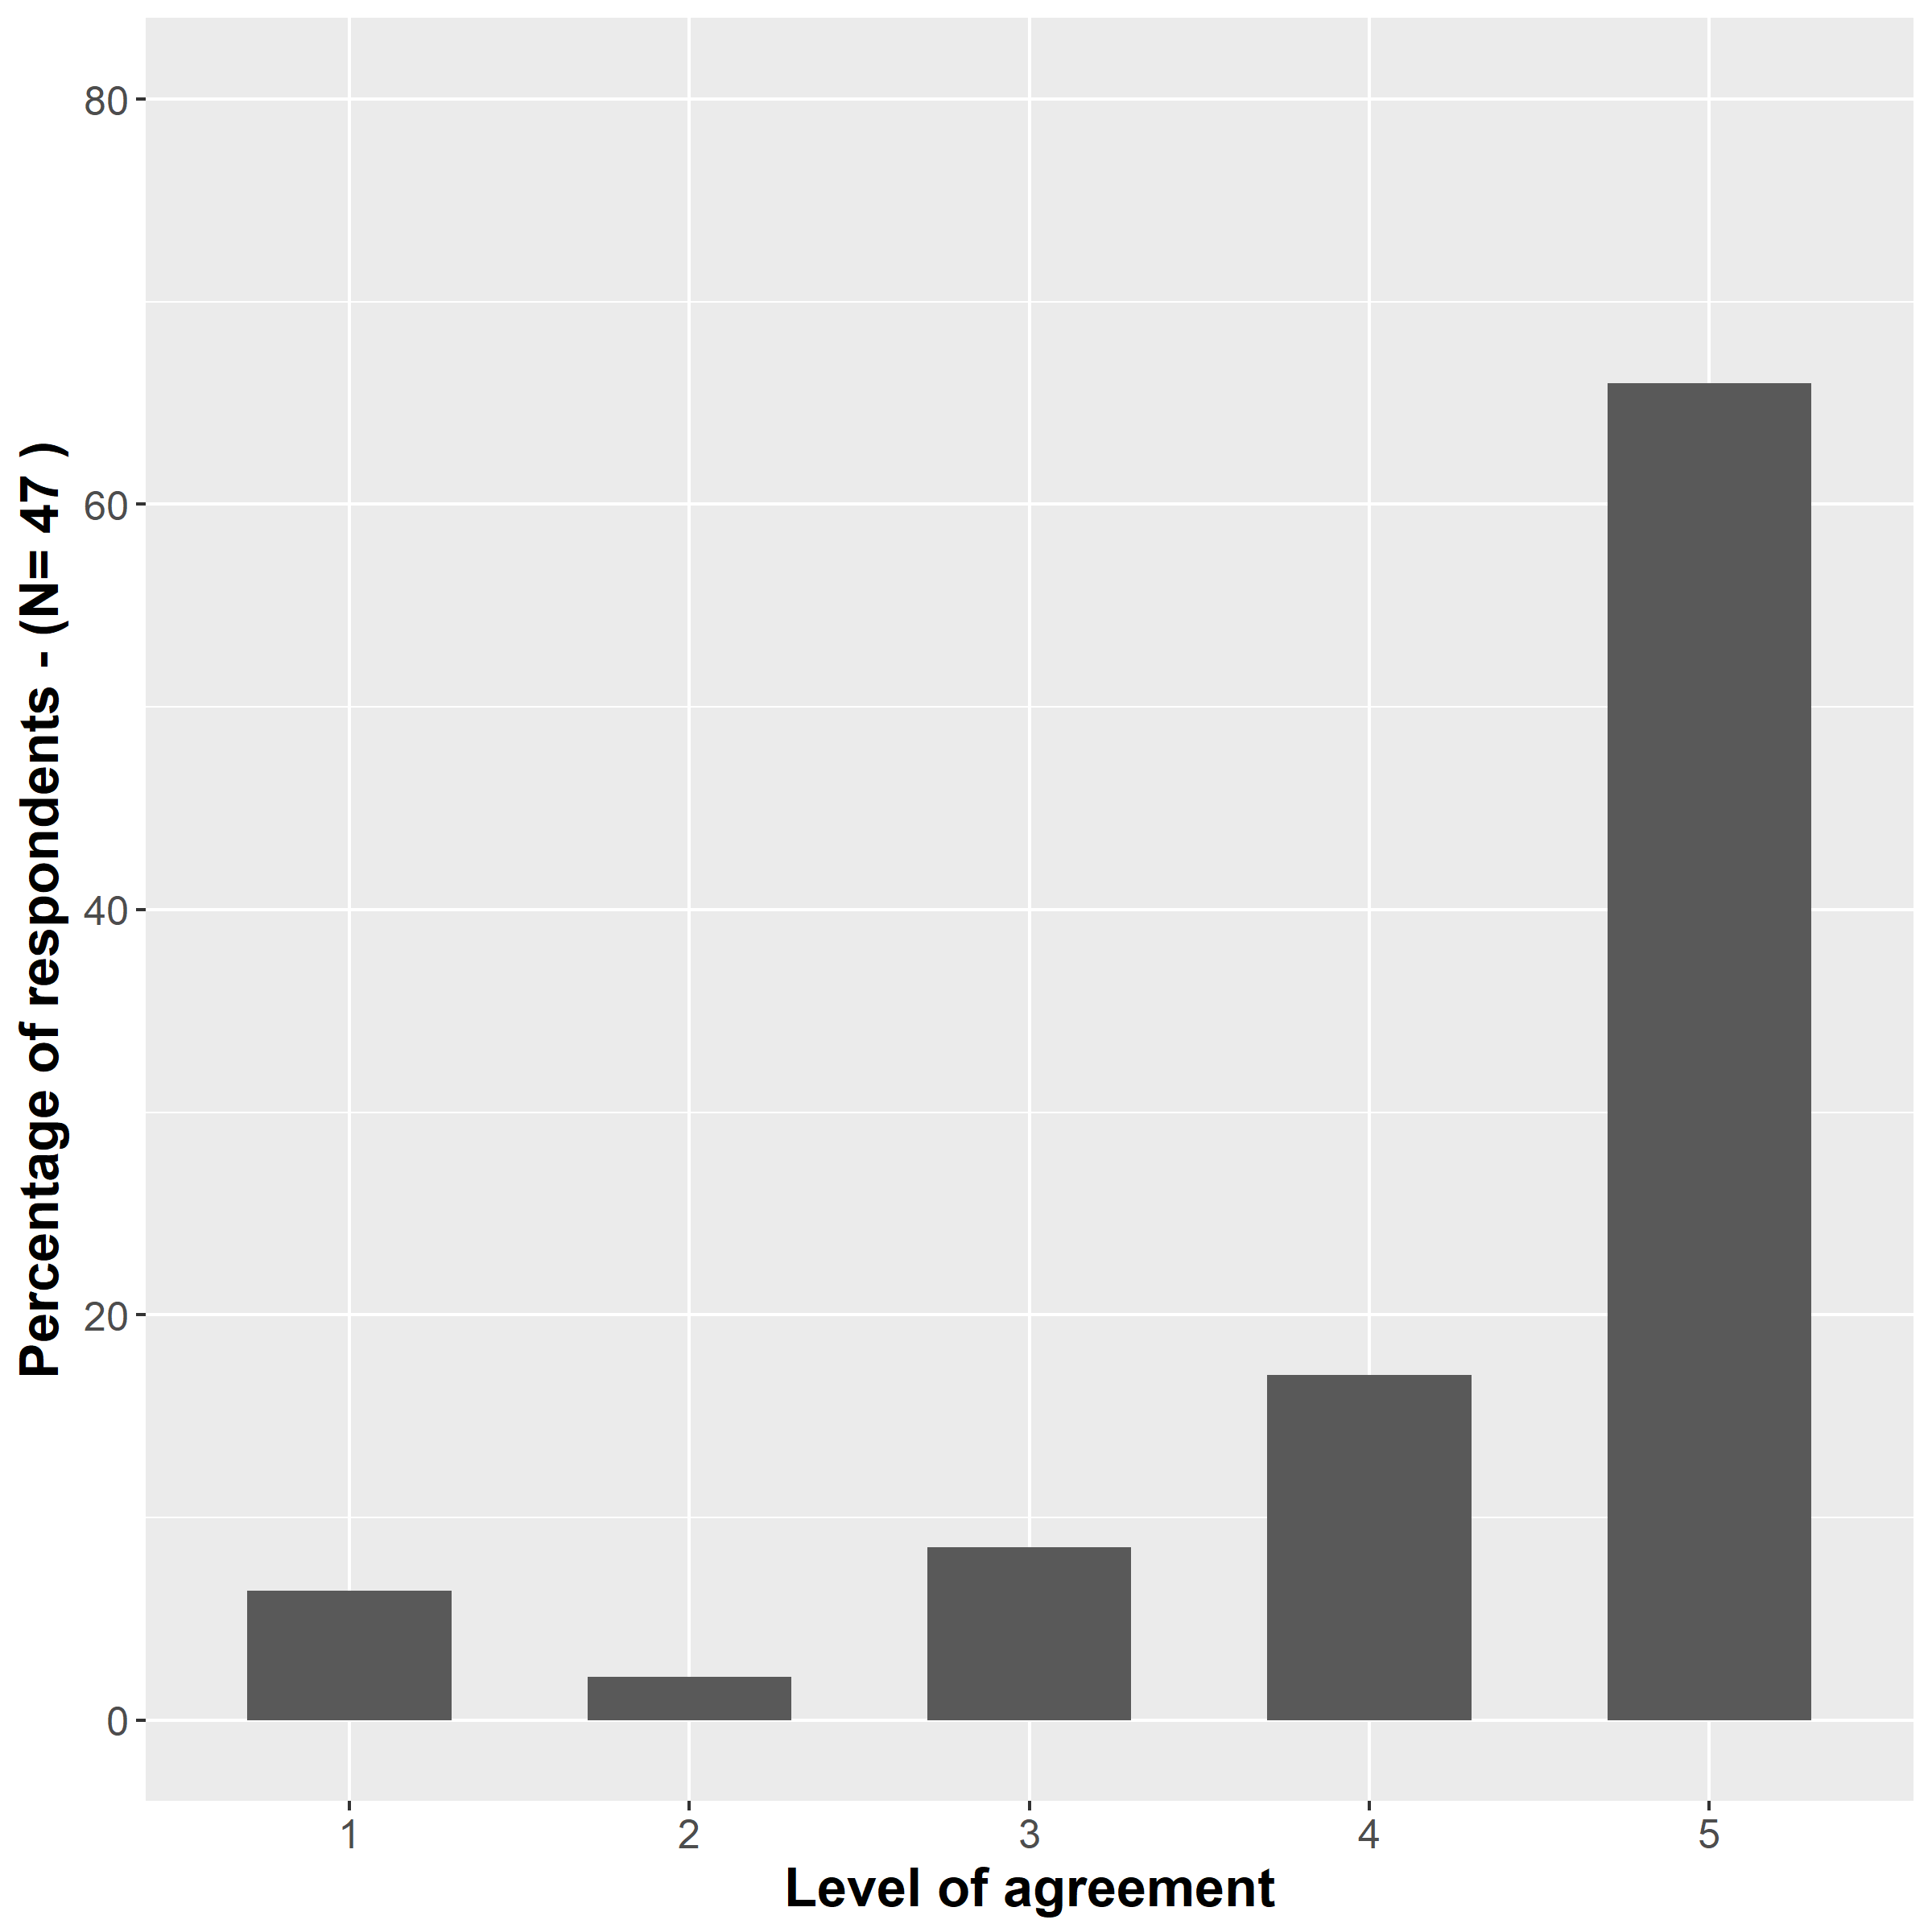
\includegraphics[width=\linewidth]{images/06-deception/staticDeceiveYoung}
    \caption{Deception - children.}
    \label{fig::staticDeceiveYoung}
  \end{subfigure} 
  %\hspace{0.01\linewidth} 
  \begin{subfigure}[t]{0.49\columnwidth}
  \centering
    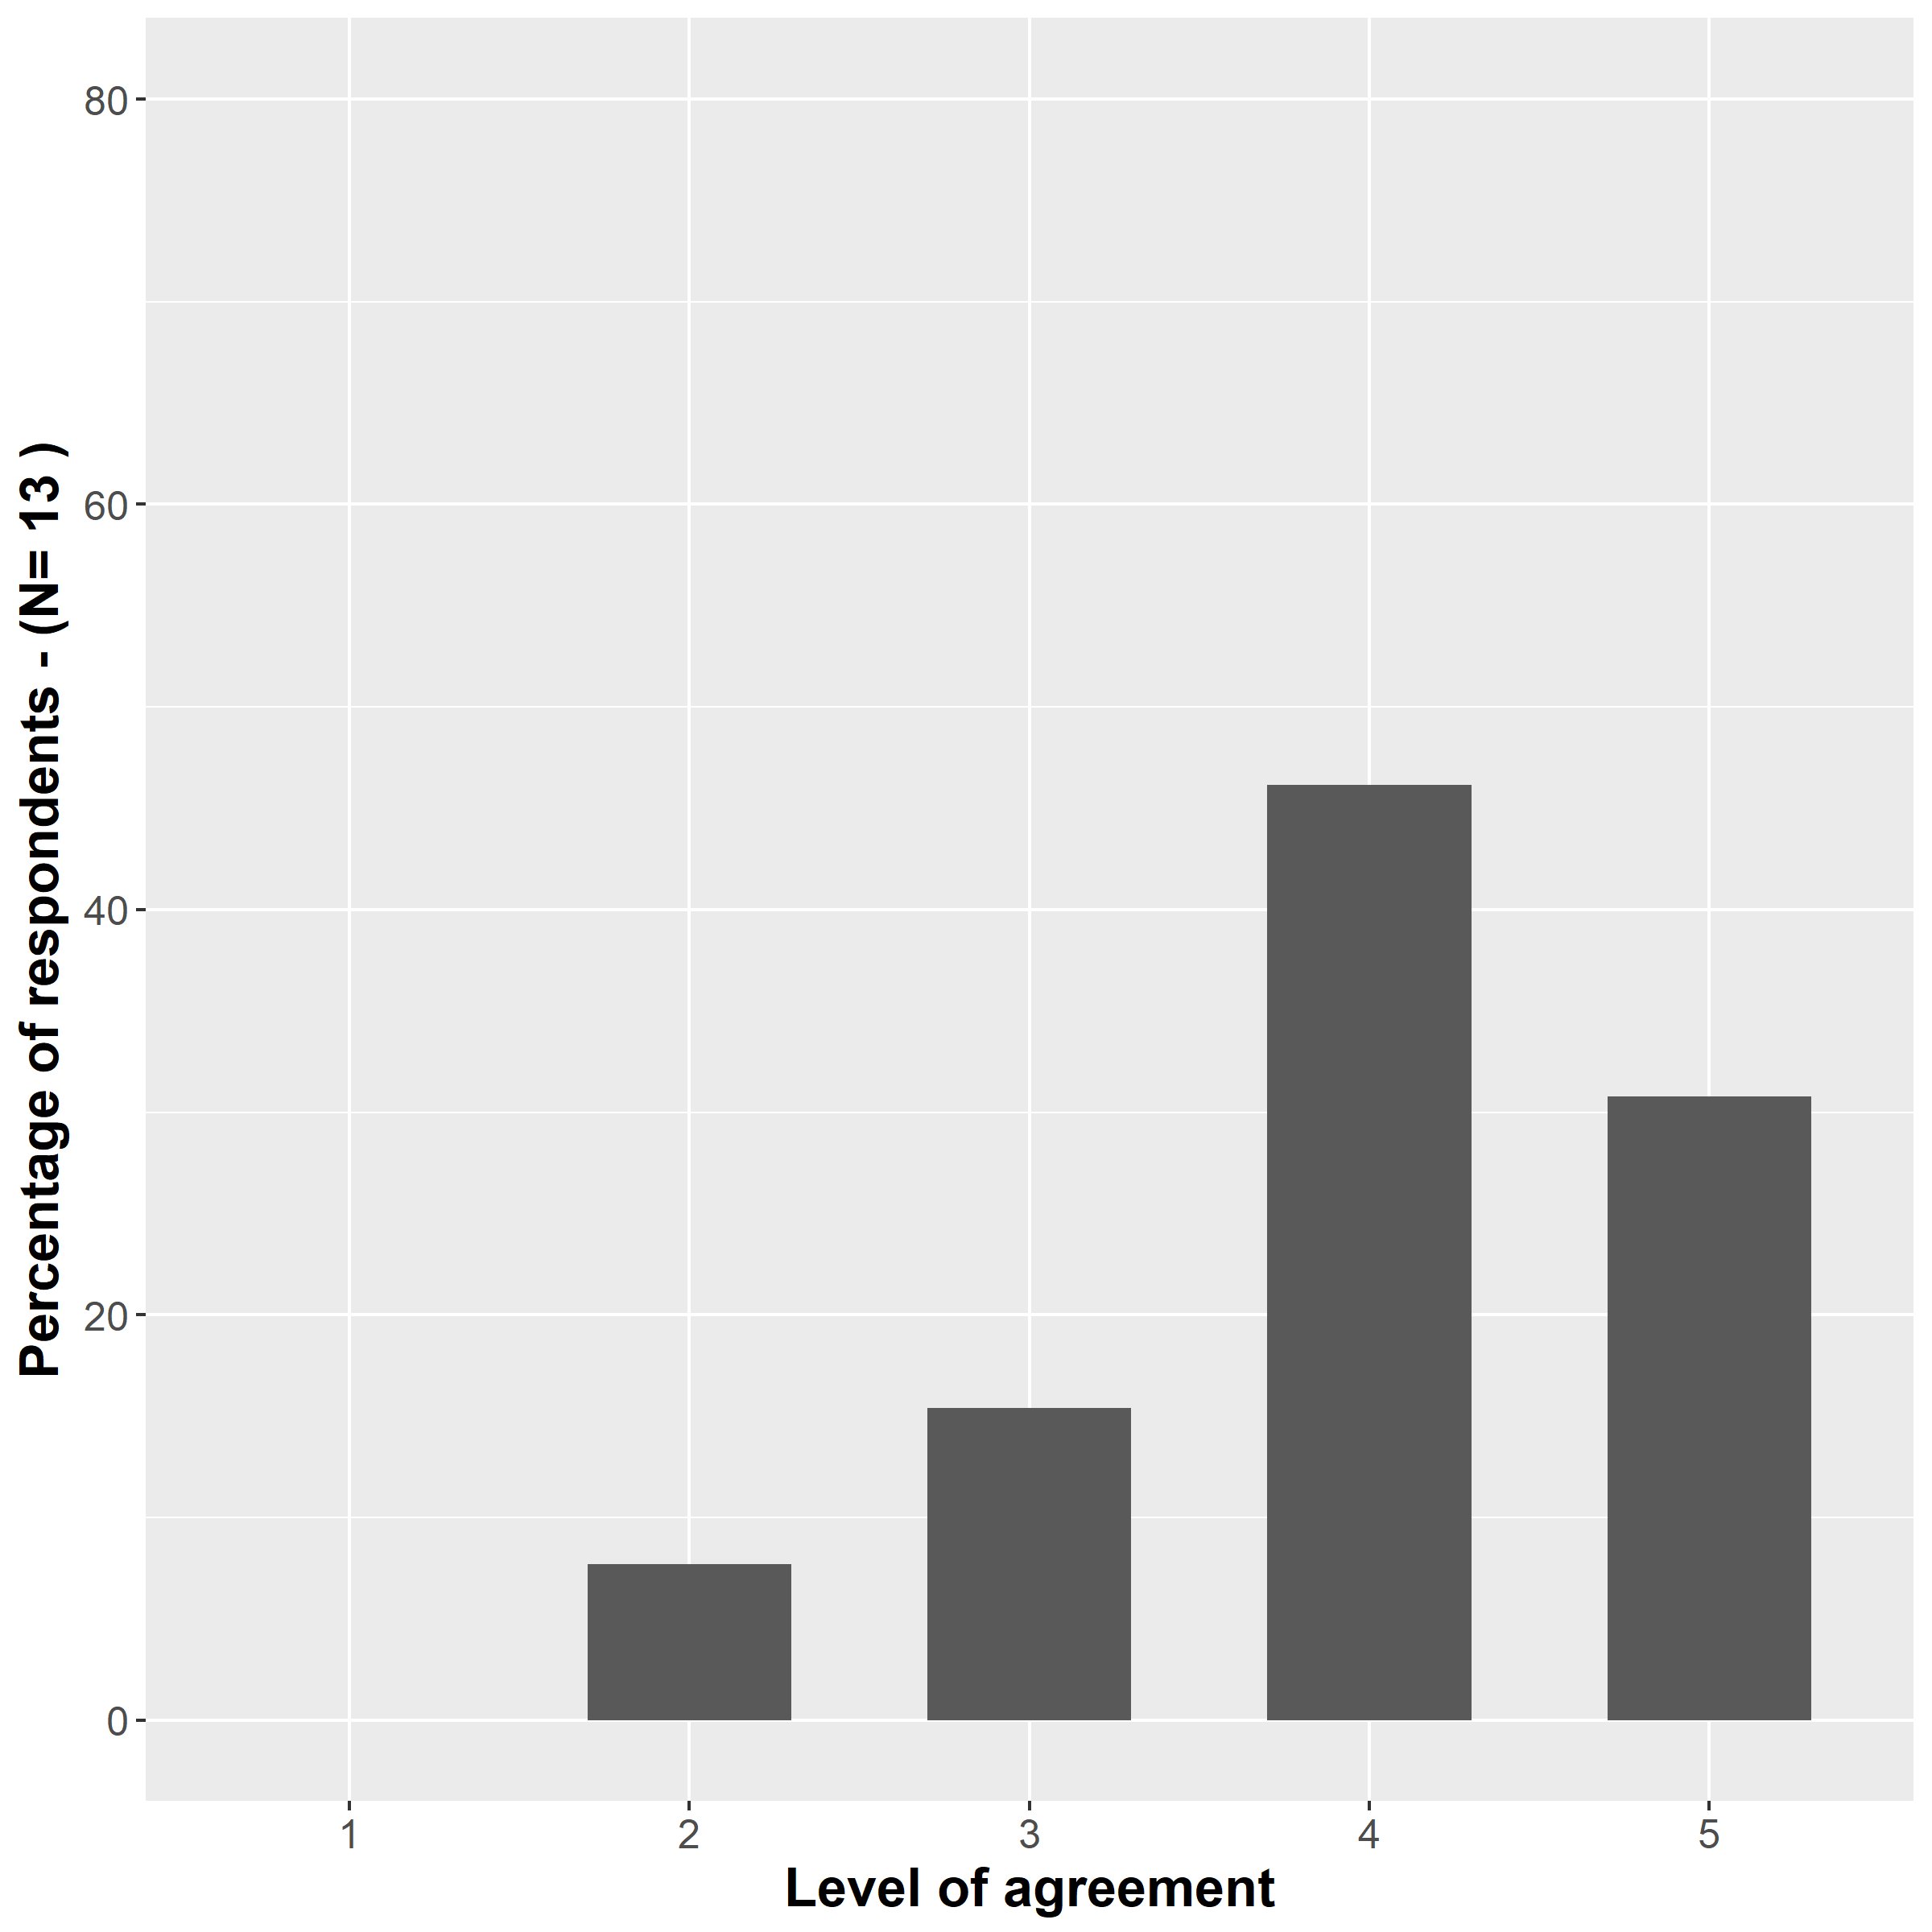
\includegraphics[width=\linewidth]{images/06-deception/staticDeceiveAdults}
    \caption{Deception - adults.}
    \label{fig::staticDeceiveAdults}
  \end{subfigure}
  \caption{Distribution of the agreement with the statement "The game was too short" ((a), (b))."The robot aimed at winning" ((c), (d)). "The robot was deceiving" ((e), (f))  1=Fully disagree 2=Disagree 3=Indifferent 4=Agree 5=Fully agree}
\end{figure*}

\subsection{Results}
All the subjects either agreed or strongly agreed with the statement: "I have enjoyed the game" (median = "strongly agree").

\subsubsection{Static deceiving strategy}
The distribution of the answers to the question: "Was the game too short?" aimed at evaluating the effort to  participate to the game, is reported in Figures~\ref{fig::staticTooShortYoung} and~\ref{fig::staticTooShortAdults}

The distribution of the agreement with the statement: "The robot aimed at winning", aimed at evaluating the perception of playing against a rational agent, is reported in Figures~\ref{fig::staticWinYoung} and~\ref{fig::staticWinAdults}.

The distribution of the agreement with the statement: "The robot was deceiving", aimed at the perception of the deceiving strategy, is reported in Figures~\ref{fig::staticDeceiveYoung} and~\ref{fig::staticDeceiveAdults}.

\subsubsection{Dynamic deceiving strategy}
The number of adult subjects playing with the dynamic deception strategy active was too small to be considered, so we report in this section only data concerning young subjects.

The distribution of the agreement to the statement: "The game was too short" aimed at evaluating the effort to  participate to the game, is reported in Figure~\ref{fig::dynamictooShortYoung}.

\begin{figure*}[tbp]
\centering
  \begin{subfigure}[t]{0.49\columnwidth}
  \centering
    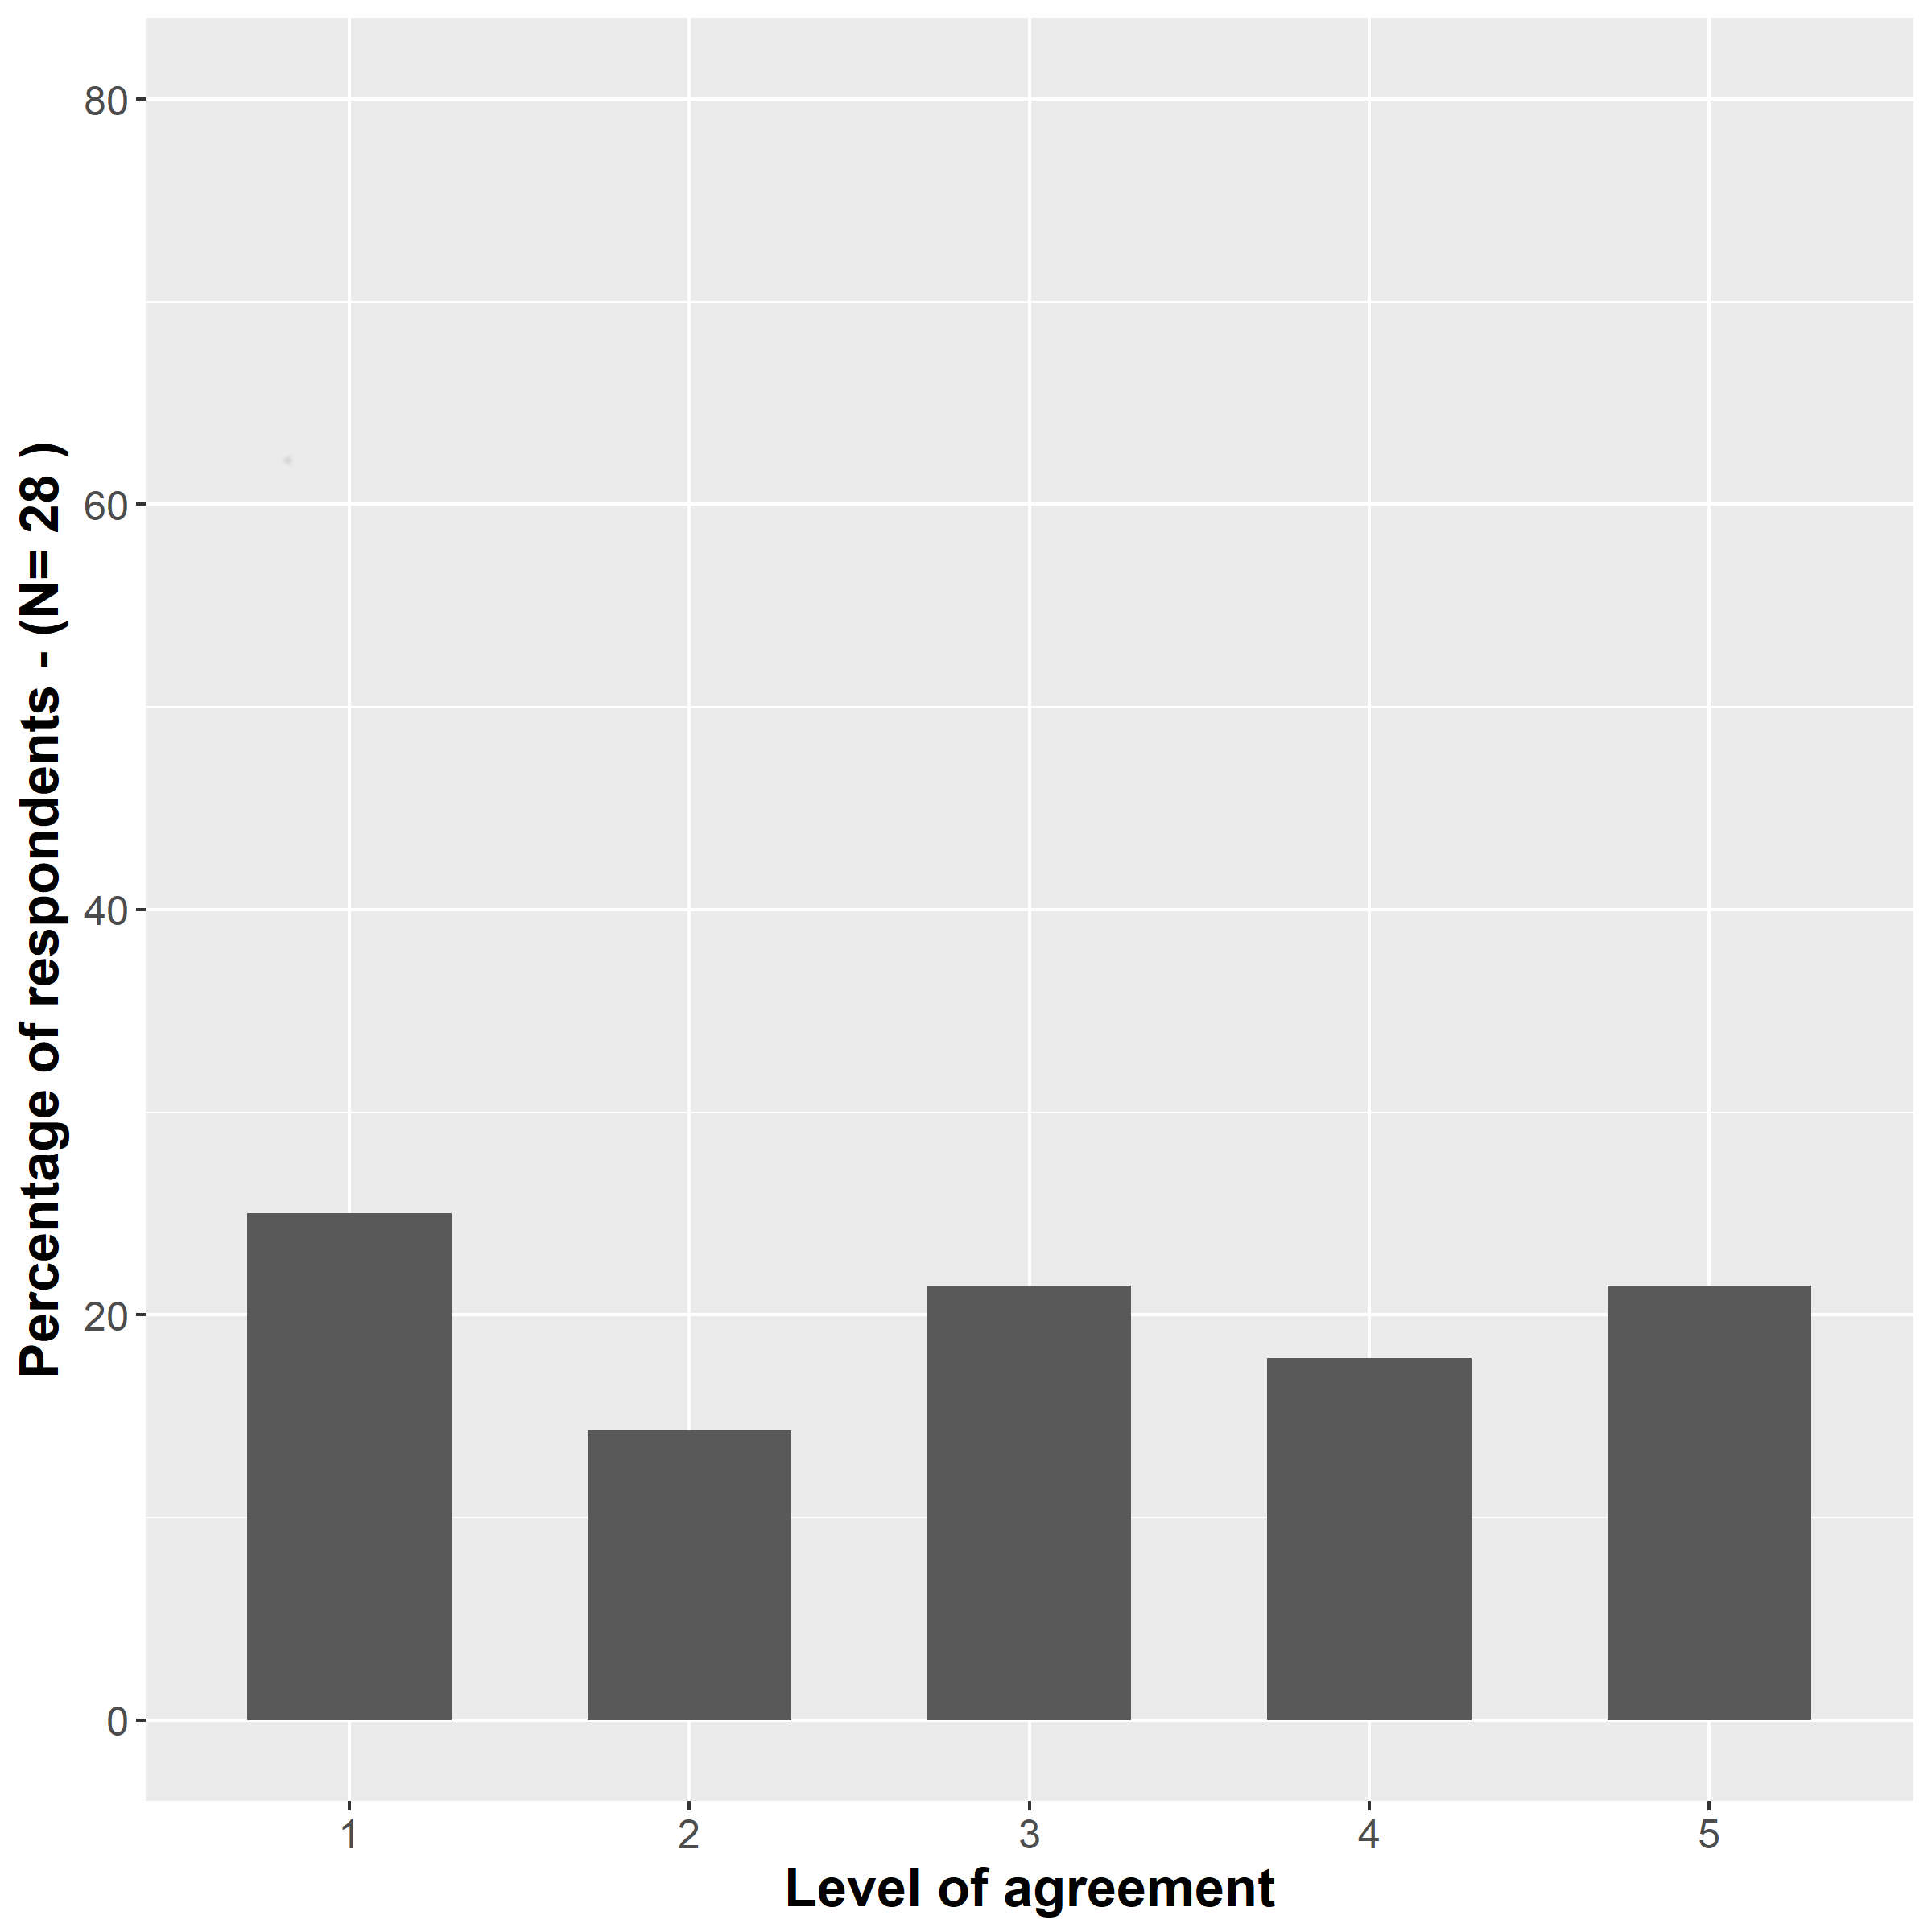
\includegraphics[width=\linewidth]{images/06-deception/dynamicTooShortYoung}
    \caption{Too short.} 
    \label{fig::dynamictooShortYoung}
  \end{subfigure}
  \hspace{0.01\columnwidth}
  \begin{subfigure}[t]{0.49\columnwidth}
  \centering
    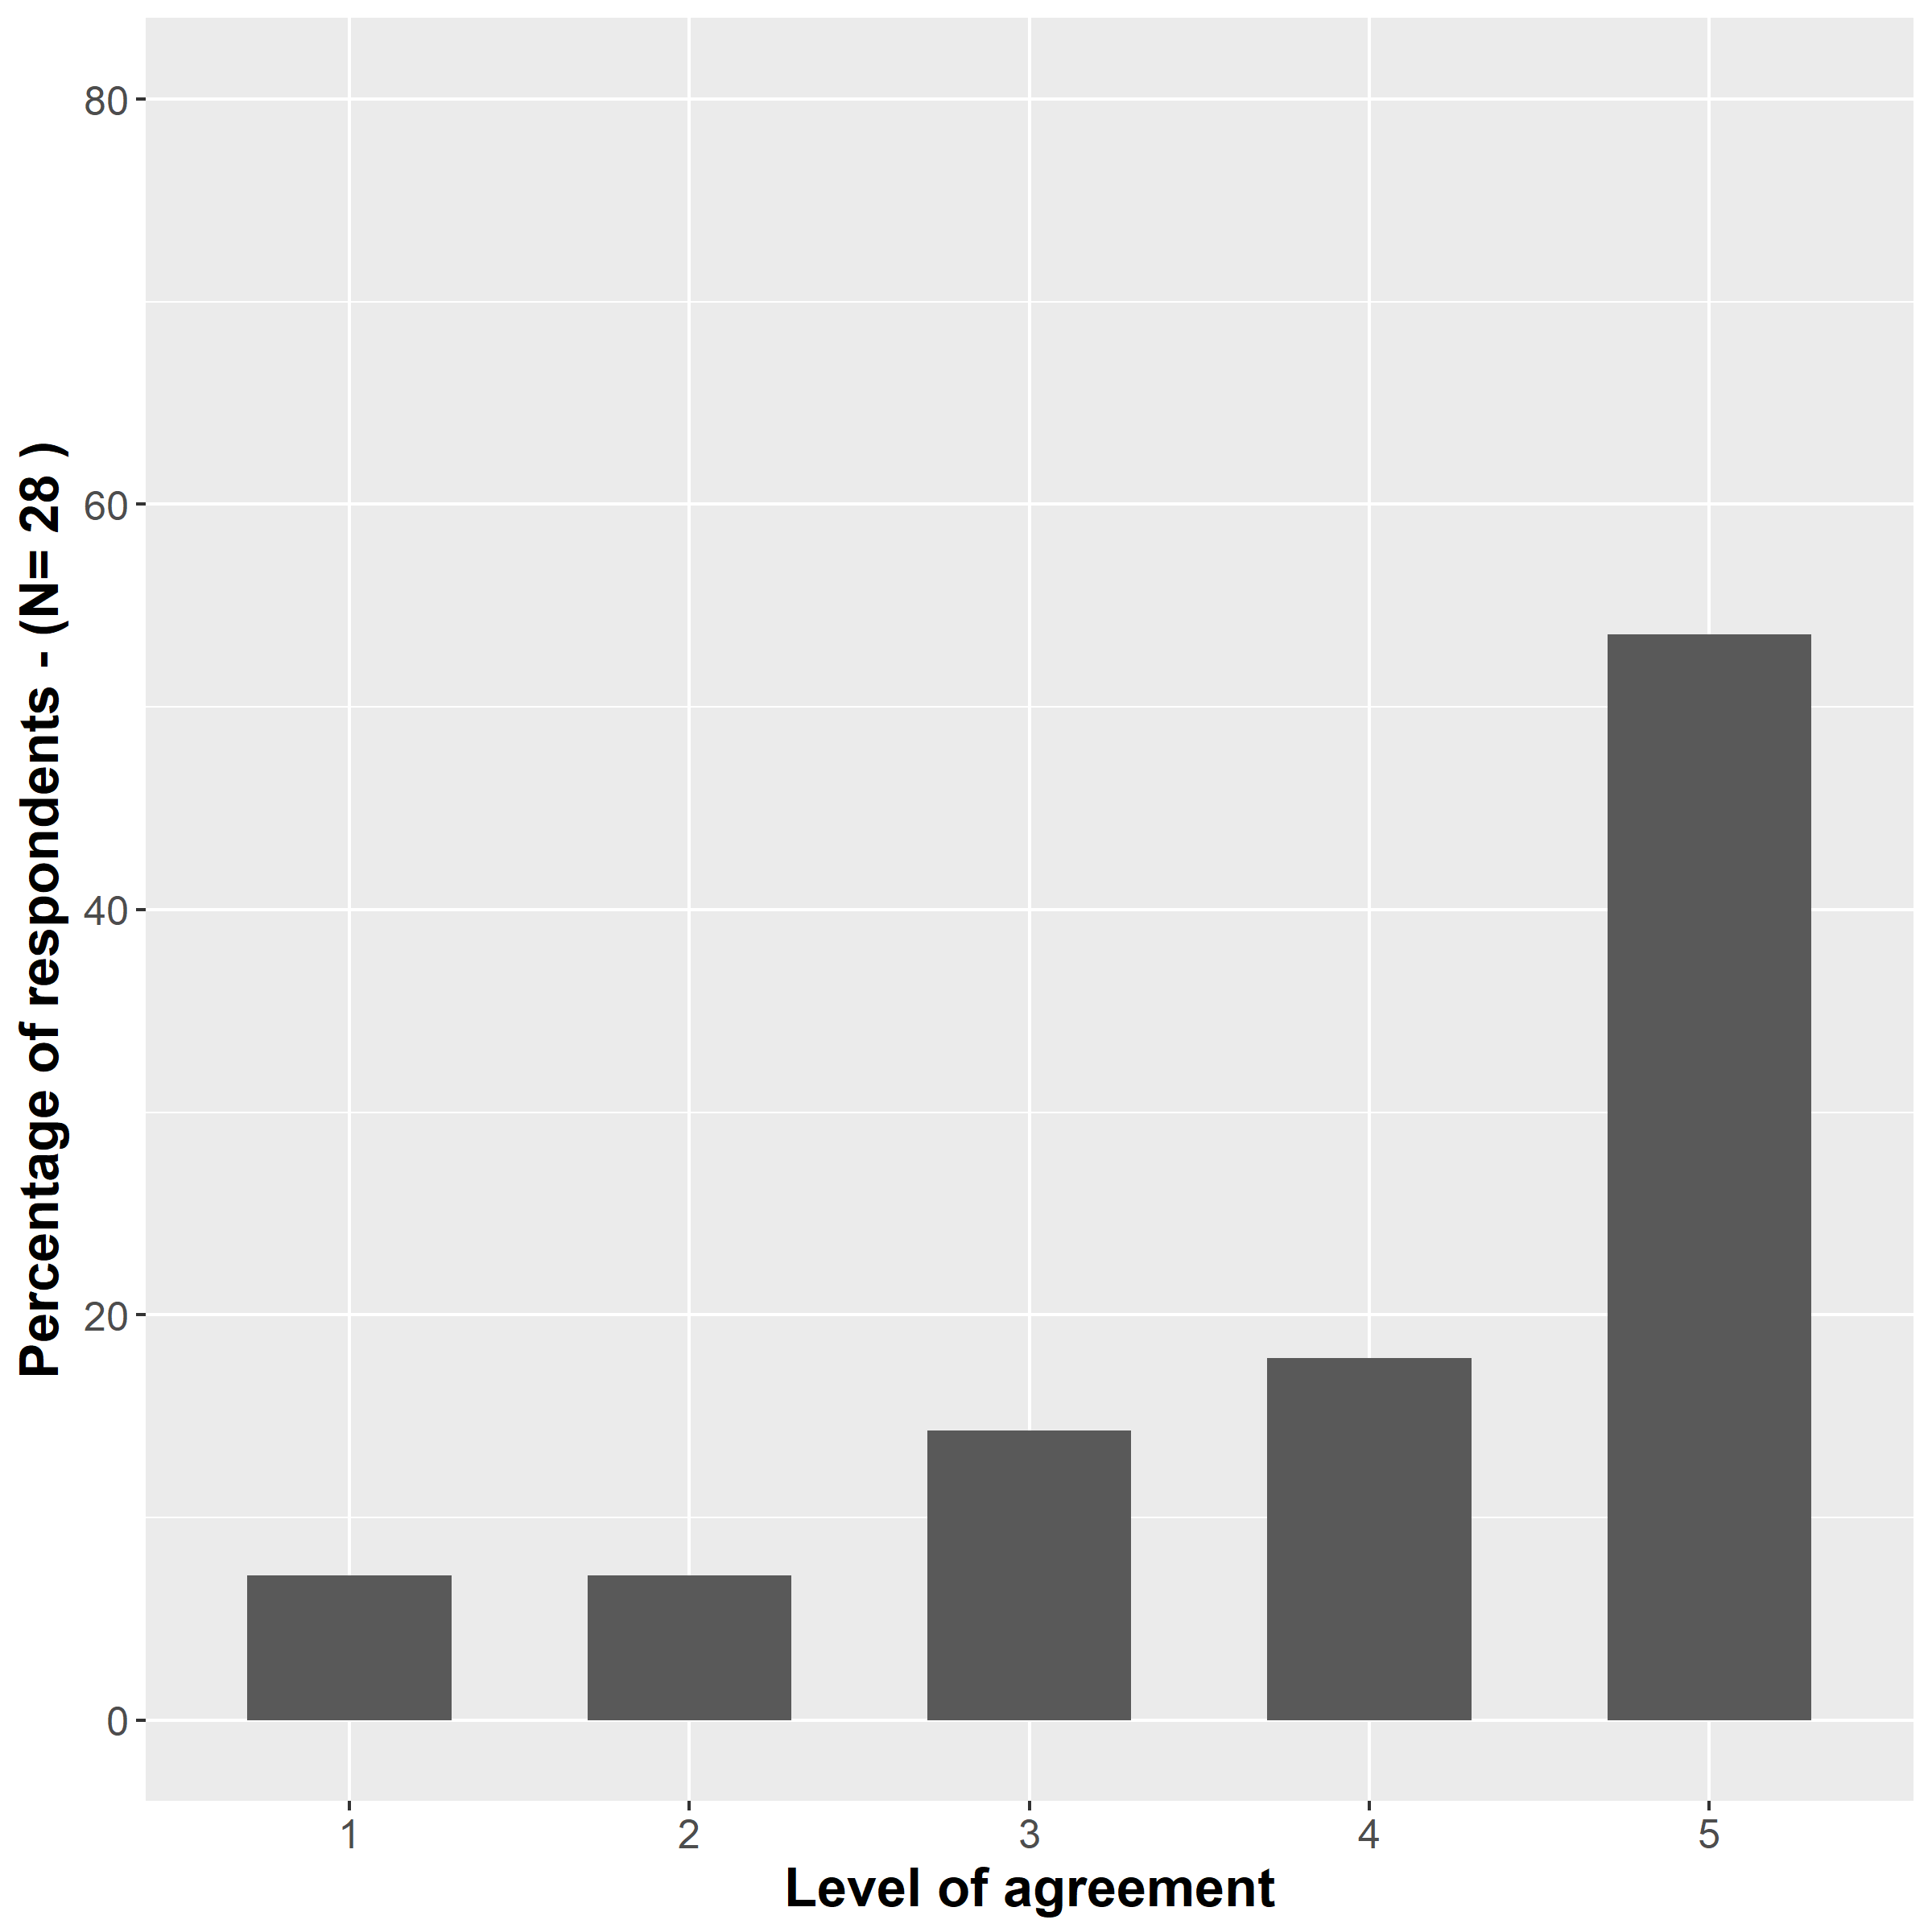
\includegraphics[width=\linewidth]{images/06-deception/dynamicWinYoung}
    \caption{Robot wants win.}
    \label{fig::dynamicWinYoung}
  \end{subfigure}
    \hspace{0.01\columnwidth}
  \begin{subfigure}[t]{0.49\columnwidth}
  \centering
    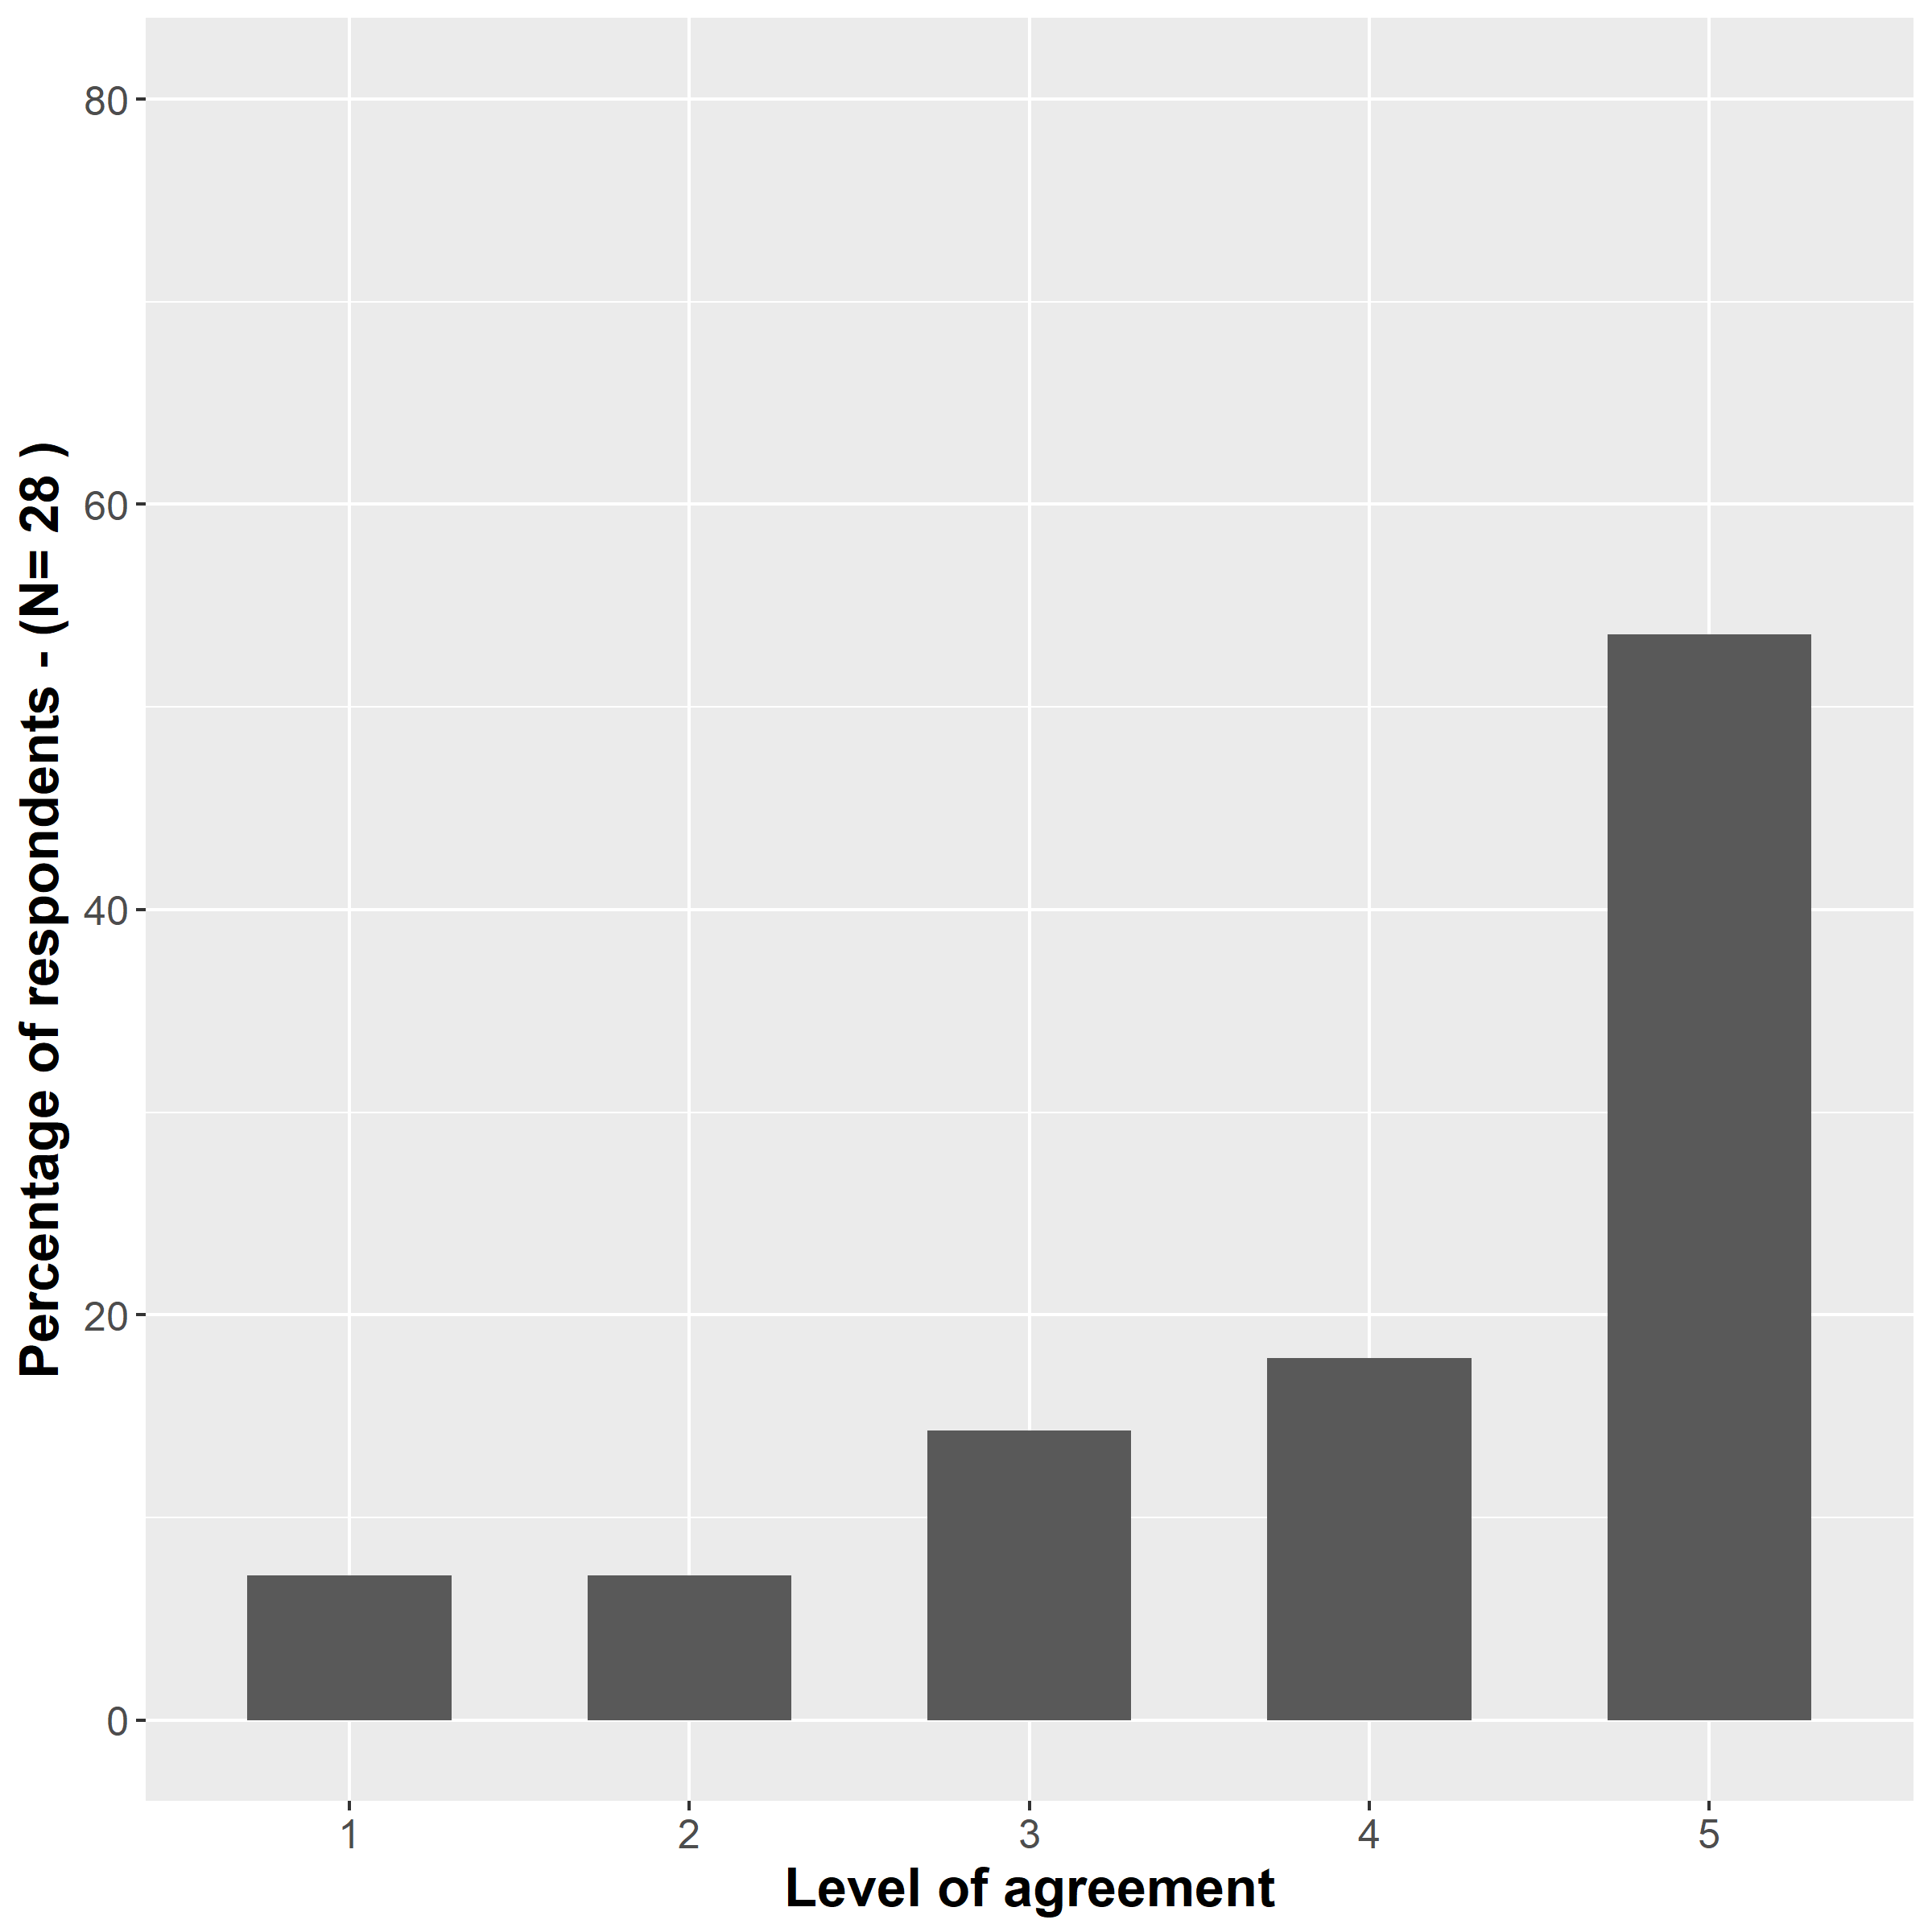
\includegraphics[width=\linewidth]{images/06-deception/dynamicWinYoung}
   \caption{Deception.}
    \label{fig::dynamicDeceiveYoung}
  \end{subfigure}
  \caption{"The game was too short" (subfig a)."The robot aimed at winning" (subfig b). "The robot was deceiving" (subfig c) 1=Fully disagree 2=Disagree 3=Indifferent 4=Agree 5=Fully agree. All subjects were children.}
\end{figure*}

The distribution of the agreement with the statement: "The robot aimed at winning", aimed at evaluating the perception of playing against a rational agent, is reported in Figure~\ref{fig::dynamicWinYoung}.

The distribution of the agreement with the statement: "The robot was deceiving",aimed at the perception of the deceiving strategy, is reported in Figure~\ref{fig::dynamicDeceiveYoung}.

\section{Discussion}
\label{S:Discussion}
We designed a game that obtained a good acceptance by all the participants, most of which queued for participating and were pleased after the game. From the values of the agreement to the statement "I have enjoyed the game", none of which was lower than "Agree", it can be said that hypothesis H1 is satisfied.  

%The length of the game was considered differently by the two classes of players with no big differences w.r.t. the different playing algorithms. It seems that adults had liked a longer play time, while children almost evenly distributed their answers among the five options.

The robot was generally perceived as a rational agent, aiming at winning the game. So we can consider hypothesis H2 as satisfied. This is a good result since the implemented strategies purposefully reduced the capabilities of the robot to adapt its behavior to match those of the players.

Furthermore, deception was perceived by most of the players, with a slightly higher number of subjects among the children strongly agreeing on the fact that the robot was actually deceiving. Hypothesis H3 can also be considered as satisfied.

No significant difference can be detected between the two algorithms in the children population, where it is possible to compare the data, so hypothesis H4 has to be rejected for this sample. Possibly, the difference between the trajectories has been washed out by the quick dynamics of the game, and the high requirement of attention to many different aspects such as the robot movement and position, the position w.r.t. the towers, and the LEDs on the towers.

\subsection{Limitations}
Among the limiting conditions of our work is the lack of a player model that can be used to tailor the deceptive motion on line. For instance, Machine Learning algorithms can be used to model the player's actions and try to maximize the level of surprise~\cite{baldi_bits_2010} regarding tower attack.
Another limitation comes from constraints that prevent quick changes in motion direction, imposed for safety reasons, which, in turn, may produce negative impacts on the perception of the deceptive movements.

\section{Conclusion and Future Works}
\label{S:Conclusion}
We have implemented a lively, enjoyable, physical robogame, where the robot is perceived as a rational agent aiming at winning the game, even if its capabilities are strongly reduced w.r.t. its possible top performance. This is an example where effective human-robot interaction is obtained by implementing robots that are not behaving optimally, in the sense of minimizing some performance parameter, but they match the expectation of interacting people to attribute rationality to the robot companion, which is one of the aims of human-robot interaction.
This result has been obtained also because of the two different deception algorithms that we have implemented, together with the system that triggers them by analyzing the game situation. These implemented deceptive trajectories are not optimal to win, but obtain the desired effect on the player. 

In the next future, we plan to collect sufficient data to perform sound statistical analyses, and to finalize a system to adapt the behavior and strategy of the robot to the perceived behavior, ability and strategies of the human players, in real time, so to optimize their satisfaction and enjoyment. 
